\subsection{Сегментация на абзацы}

Сегментация~--- процесс разделения входного изображения на отдельные области, называемые сегментами, представляющие собой уникальную часть изображения. Цель сегментатции заключается в улучшении понимании и интерпретации изображения, а также в анализе и классификации объектов на изображении.
Примером сегментации может служить распознавание машин с видеокамеры дорожного наблюдения, обнаружение дорожных знаков с видеорегистратора и т.д.

В данной работе сегментация служит для:
\begin{itemize}
    \item выделения абзацев;
    \item отделения текста от формул, рисунков и пр.
\end{itemize}

Цели являются независимыми друг от друга, поэтому их можно выделить на отдельные этапы сегментации, а также исполнять параллельно. 

Выделение абзацев требуется для дальнейшего сохранения структуры текста в \LaTeX\; коде. Данный вид сегментации, как и коррекция перспективы, осуществляется при помощи алгоритмов обработки изображения.
Поэтому данный этап можно также исполнять на ЭВМ пользователя.

Требуется понять, что такое абзац в контексте изображения. Будем считать абзацем последовательность строк текста, находящихся друг от друга на небольшом расстоянии.

\subsubsection{Сегментация изображения}

Рассмотрим алгоритм сегментации изображения на абзацы на примере изображения, представленного на рисунке ~\ref{segmentation_input}.

\begin{figure}
    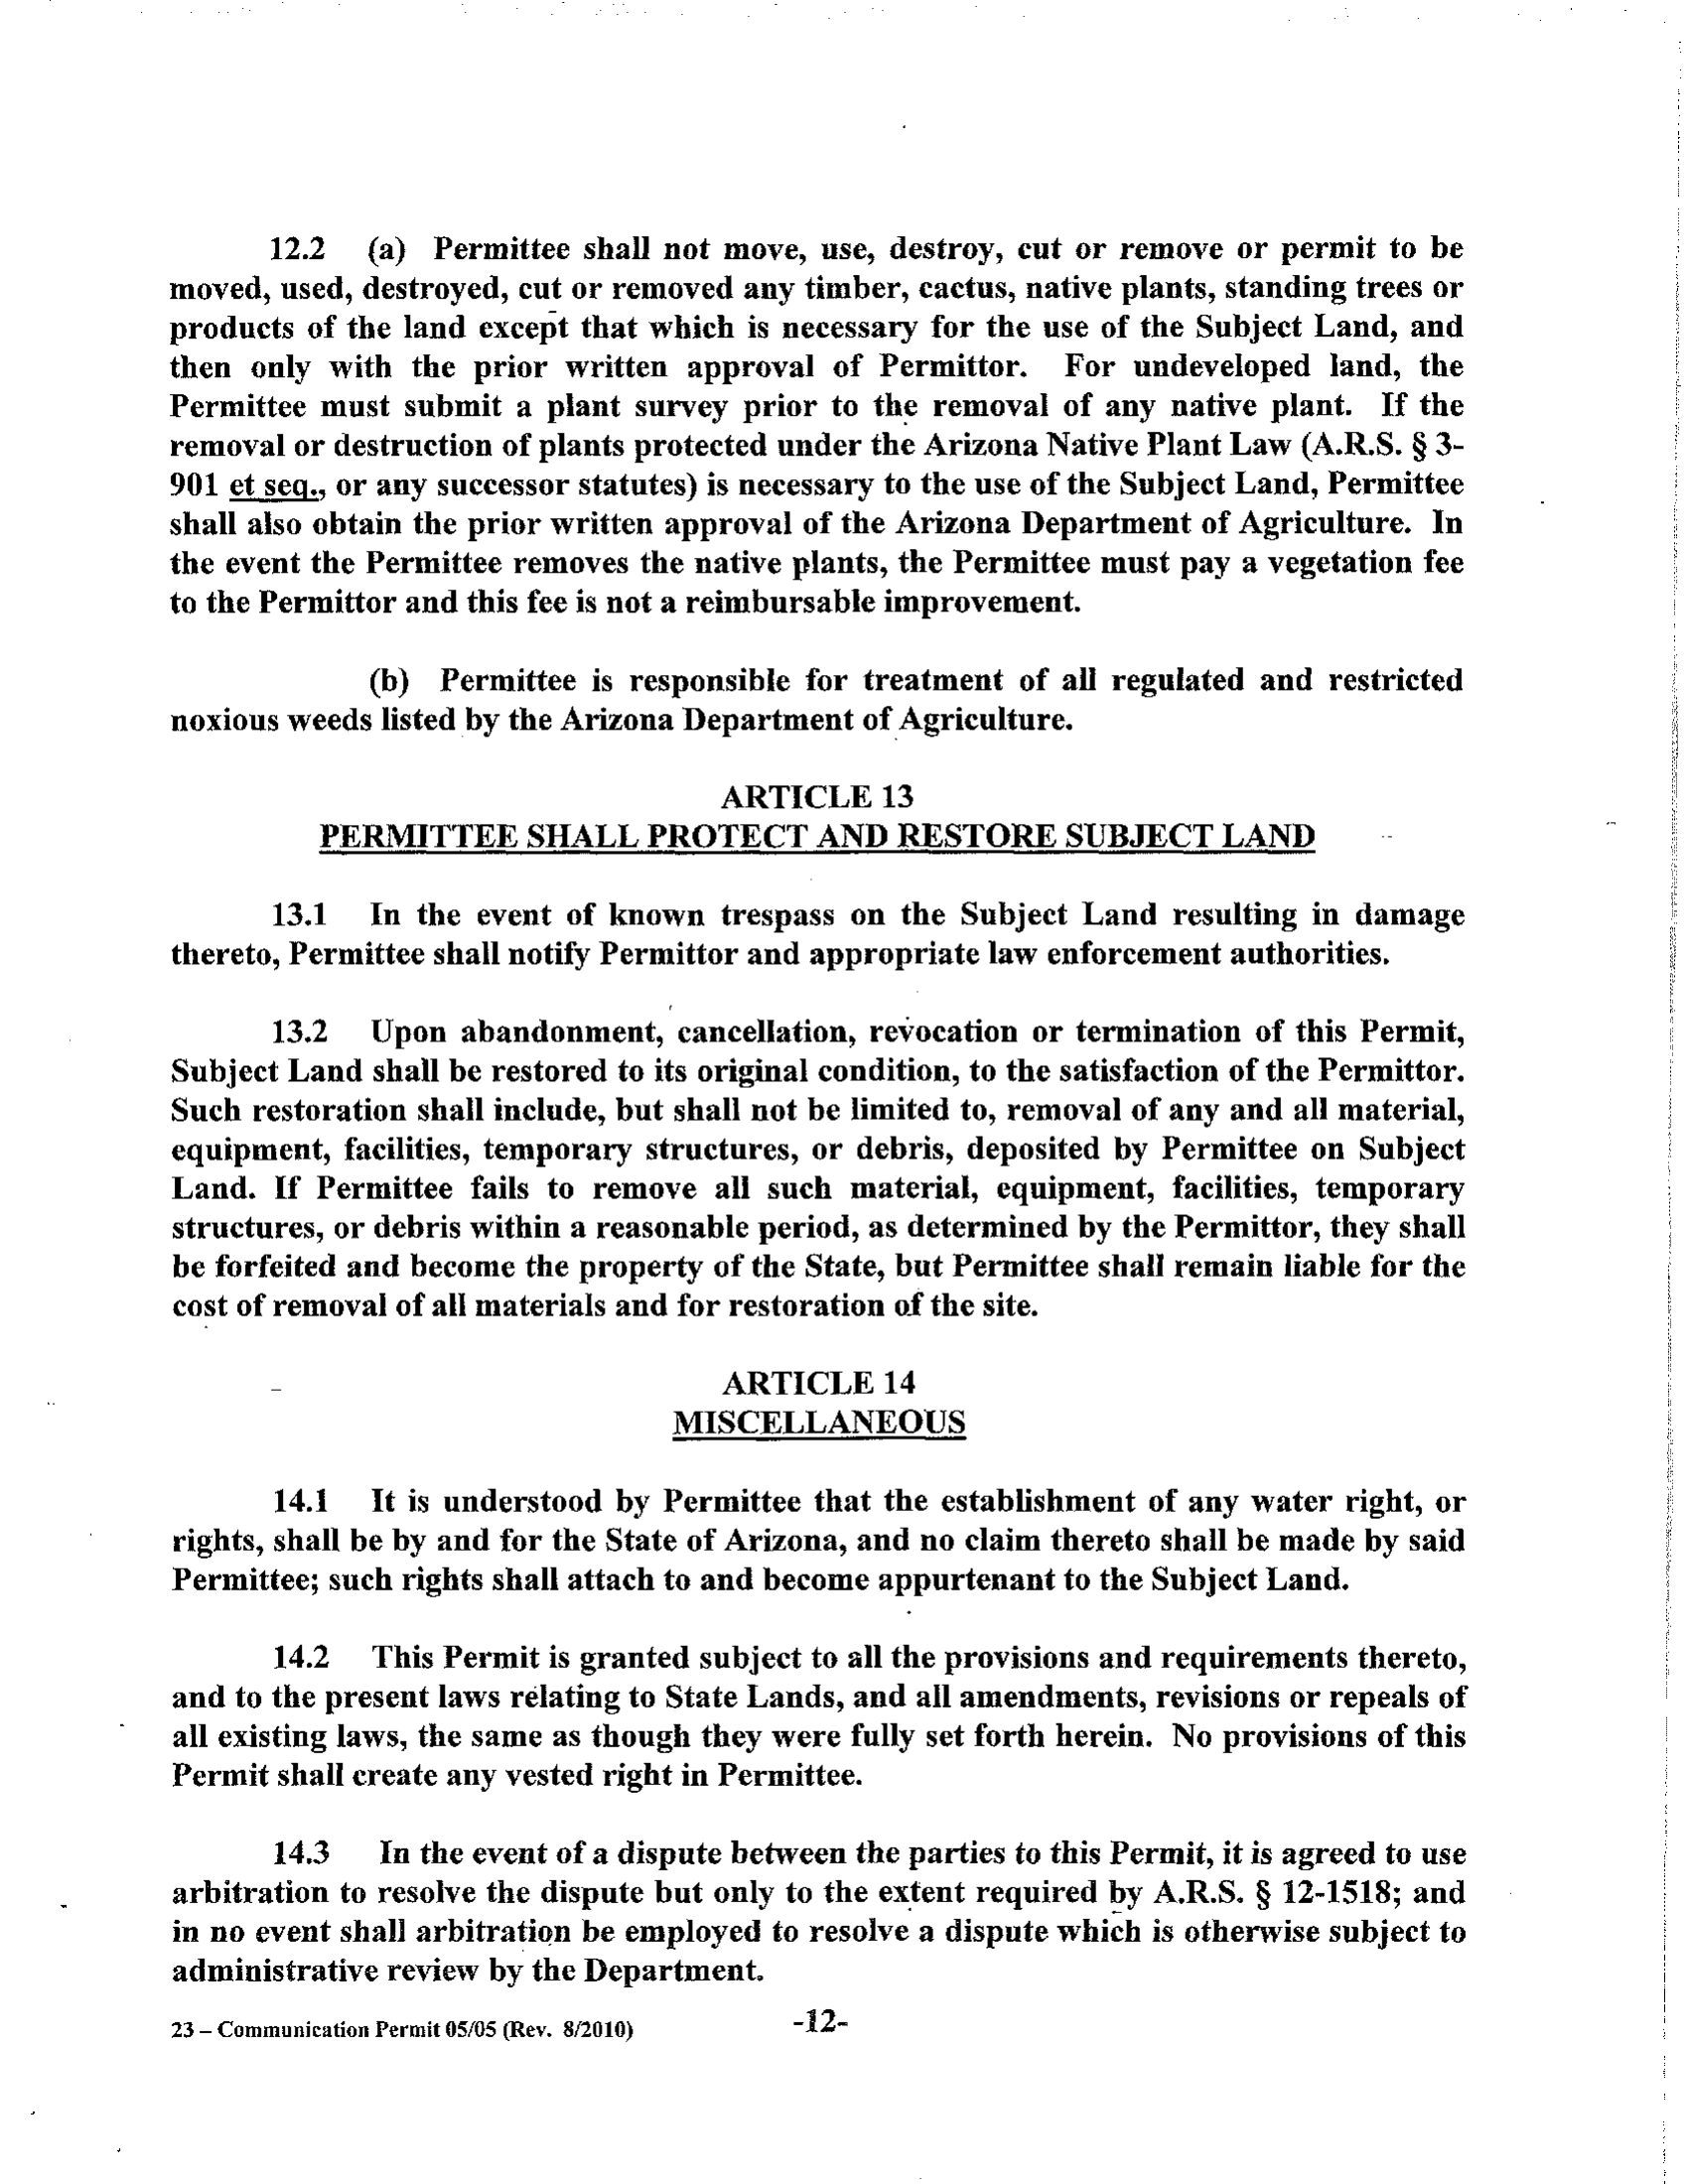
\includegraphics[scale=0.5]{img/paragraph/input.png}
    \caption{Входное изображение алгоритма}
    \label{segmentation_input}
\end{figure}

Сначала необходимо бинаризовать изображение. Для этого используется размытие Гаусса \cite{gauss_blur}, представленное на рисунке ~\ref{segmentation_blur}, а затем преобразование Трешхолда \cite{opencv_threshold}, представленное на рисунке ~\ref{segmentation_threshold}.

\begin{figure}
    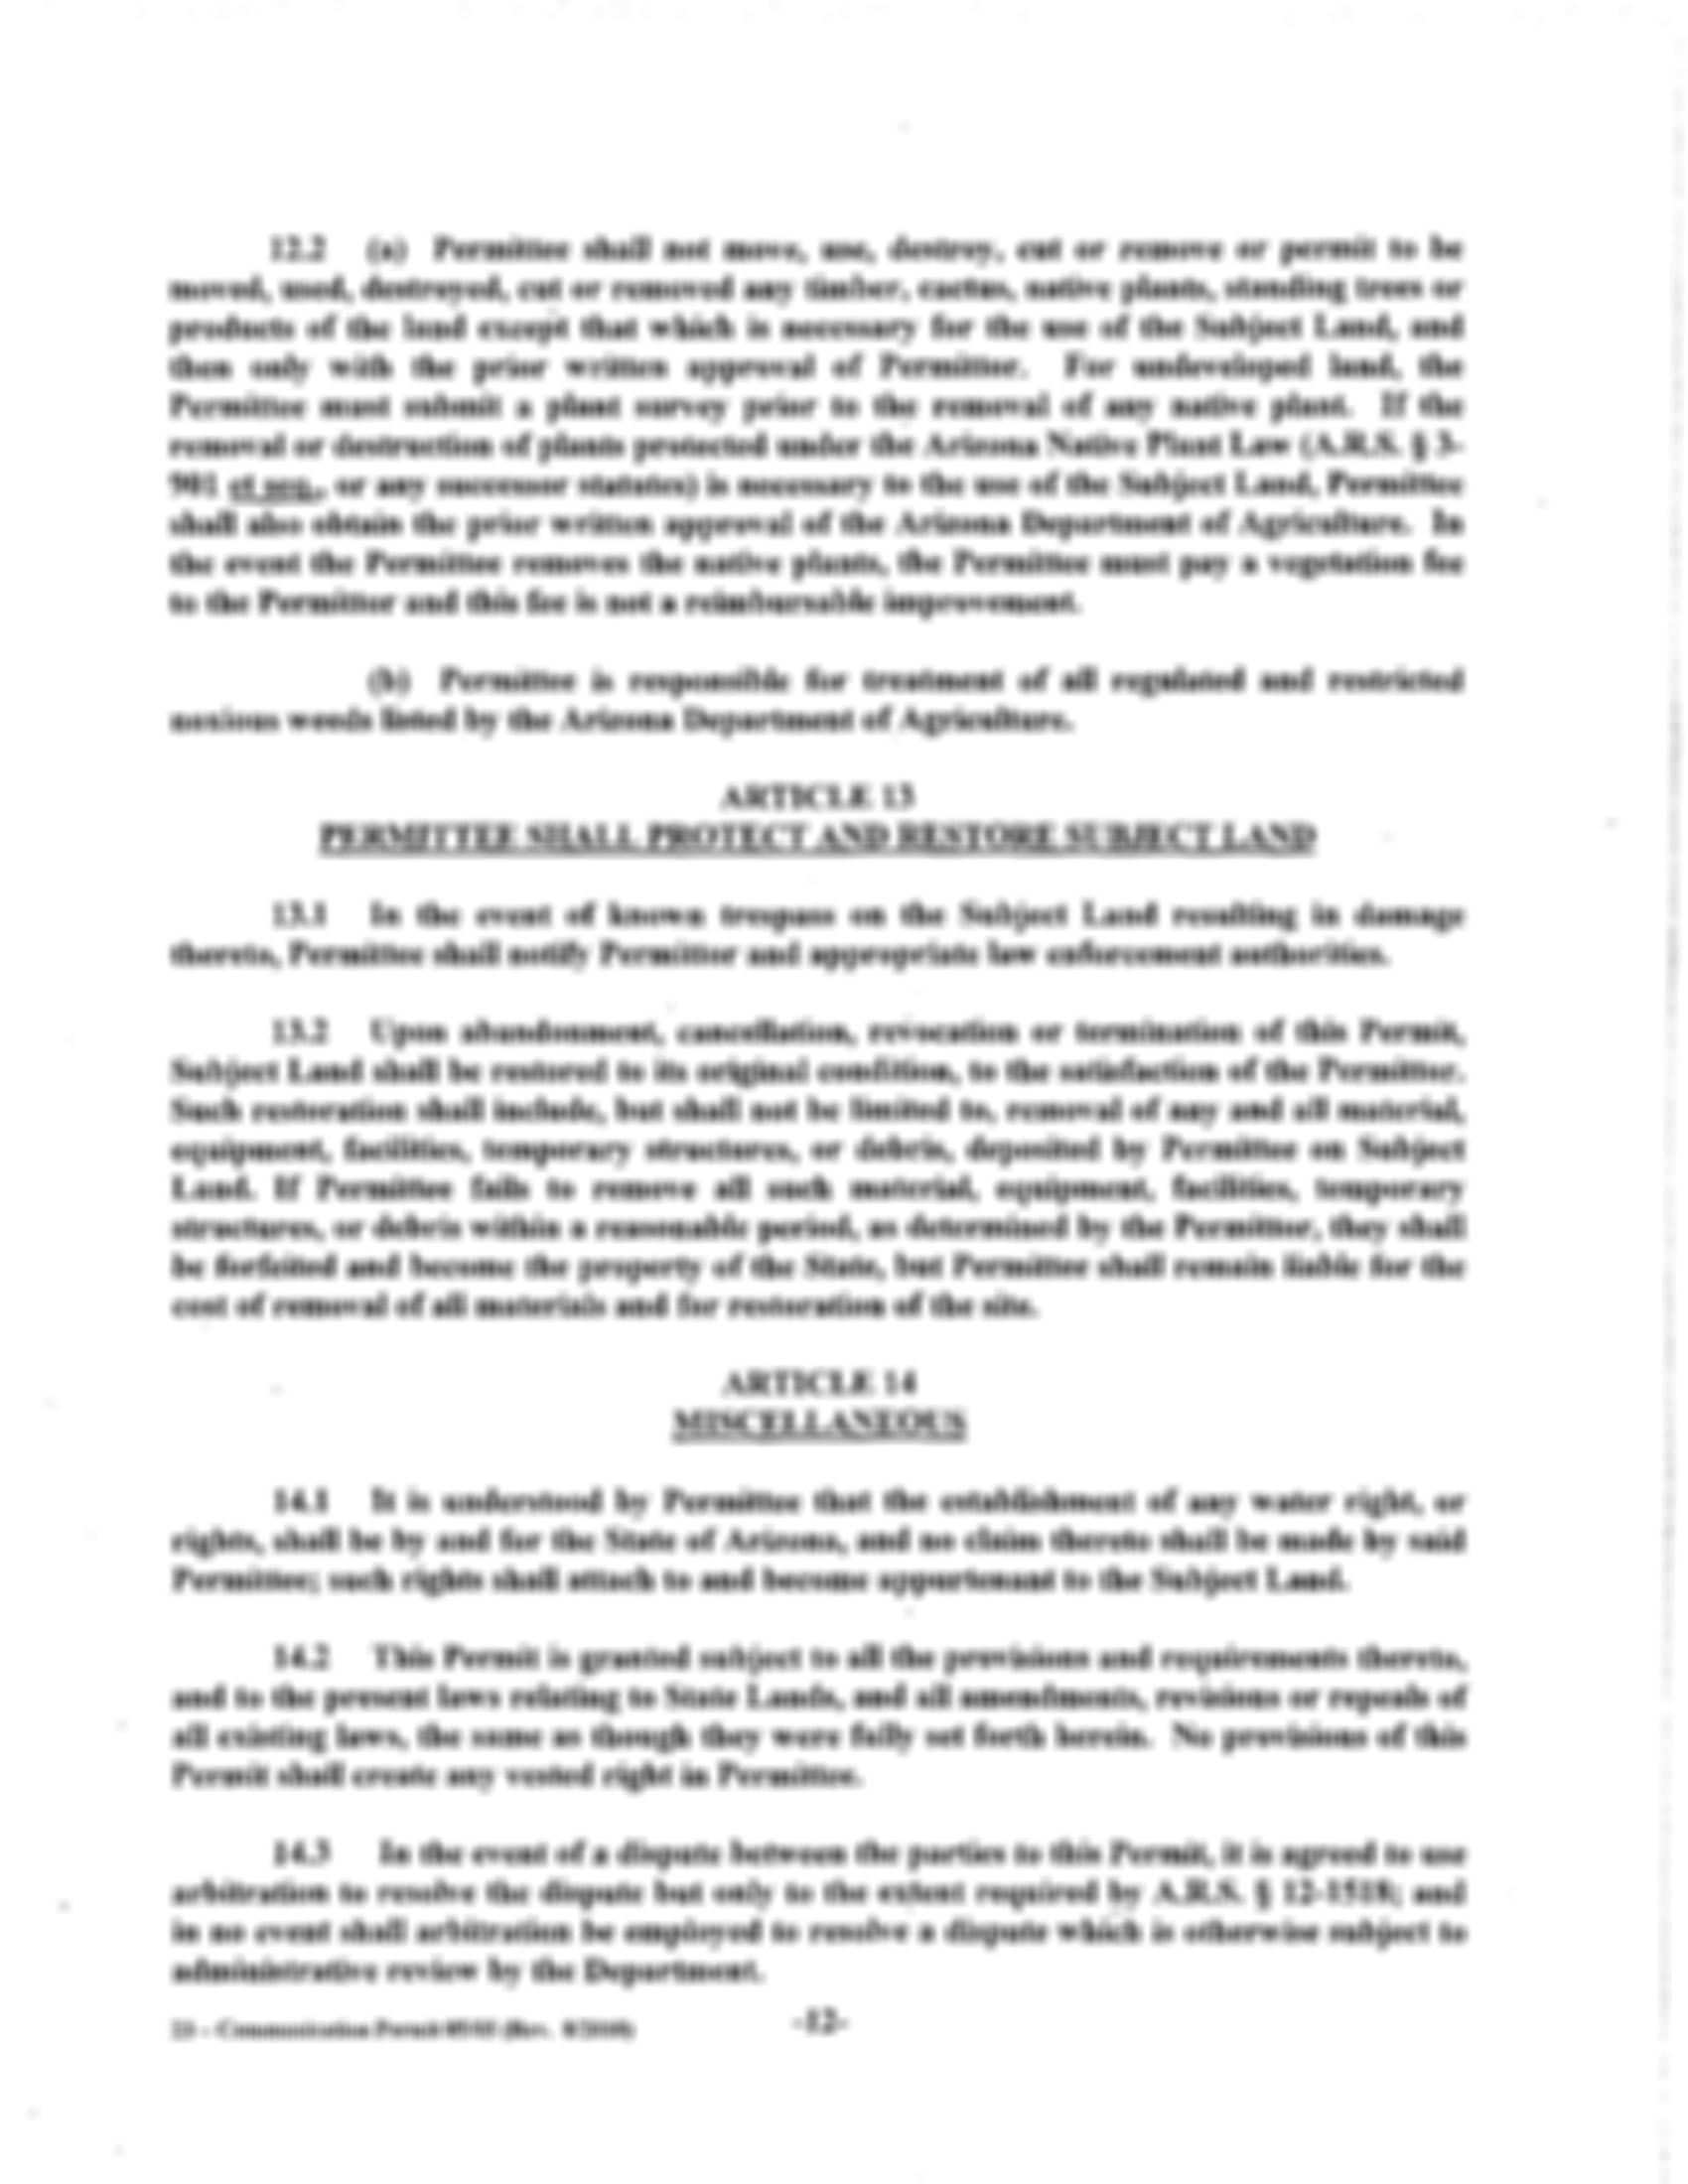
\includegraphics[scale=0.2]{img/paragraph/blur.png}
    \caption{Изображение после размытия Гаусса}
    \label{segmentation_blur}
\end{figure}

\begin{figure}
    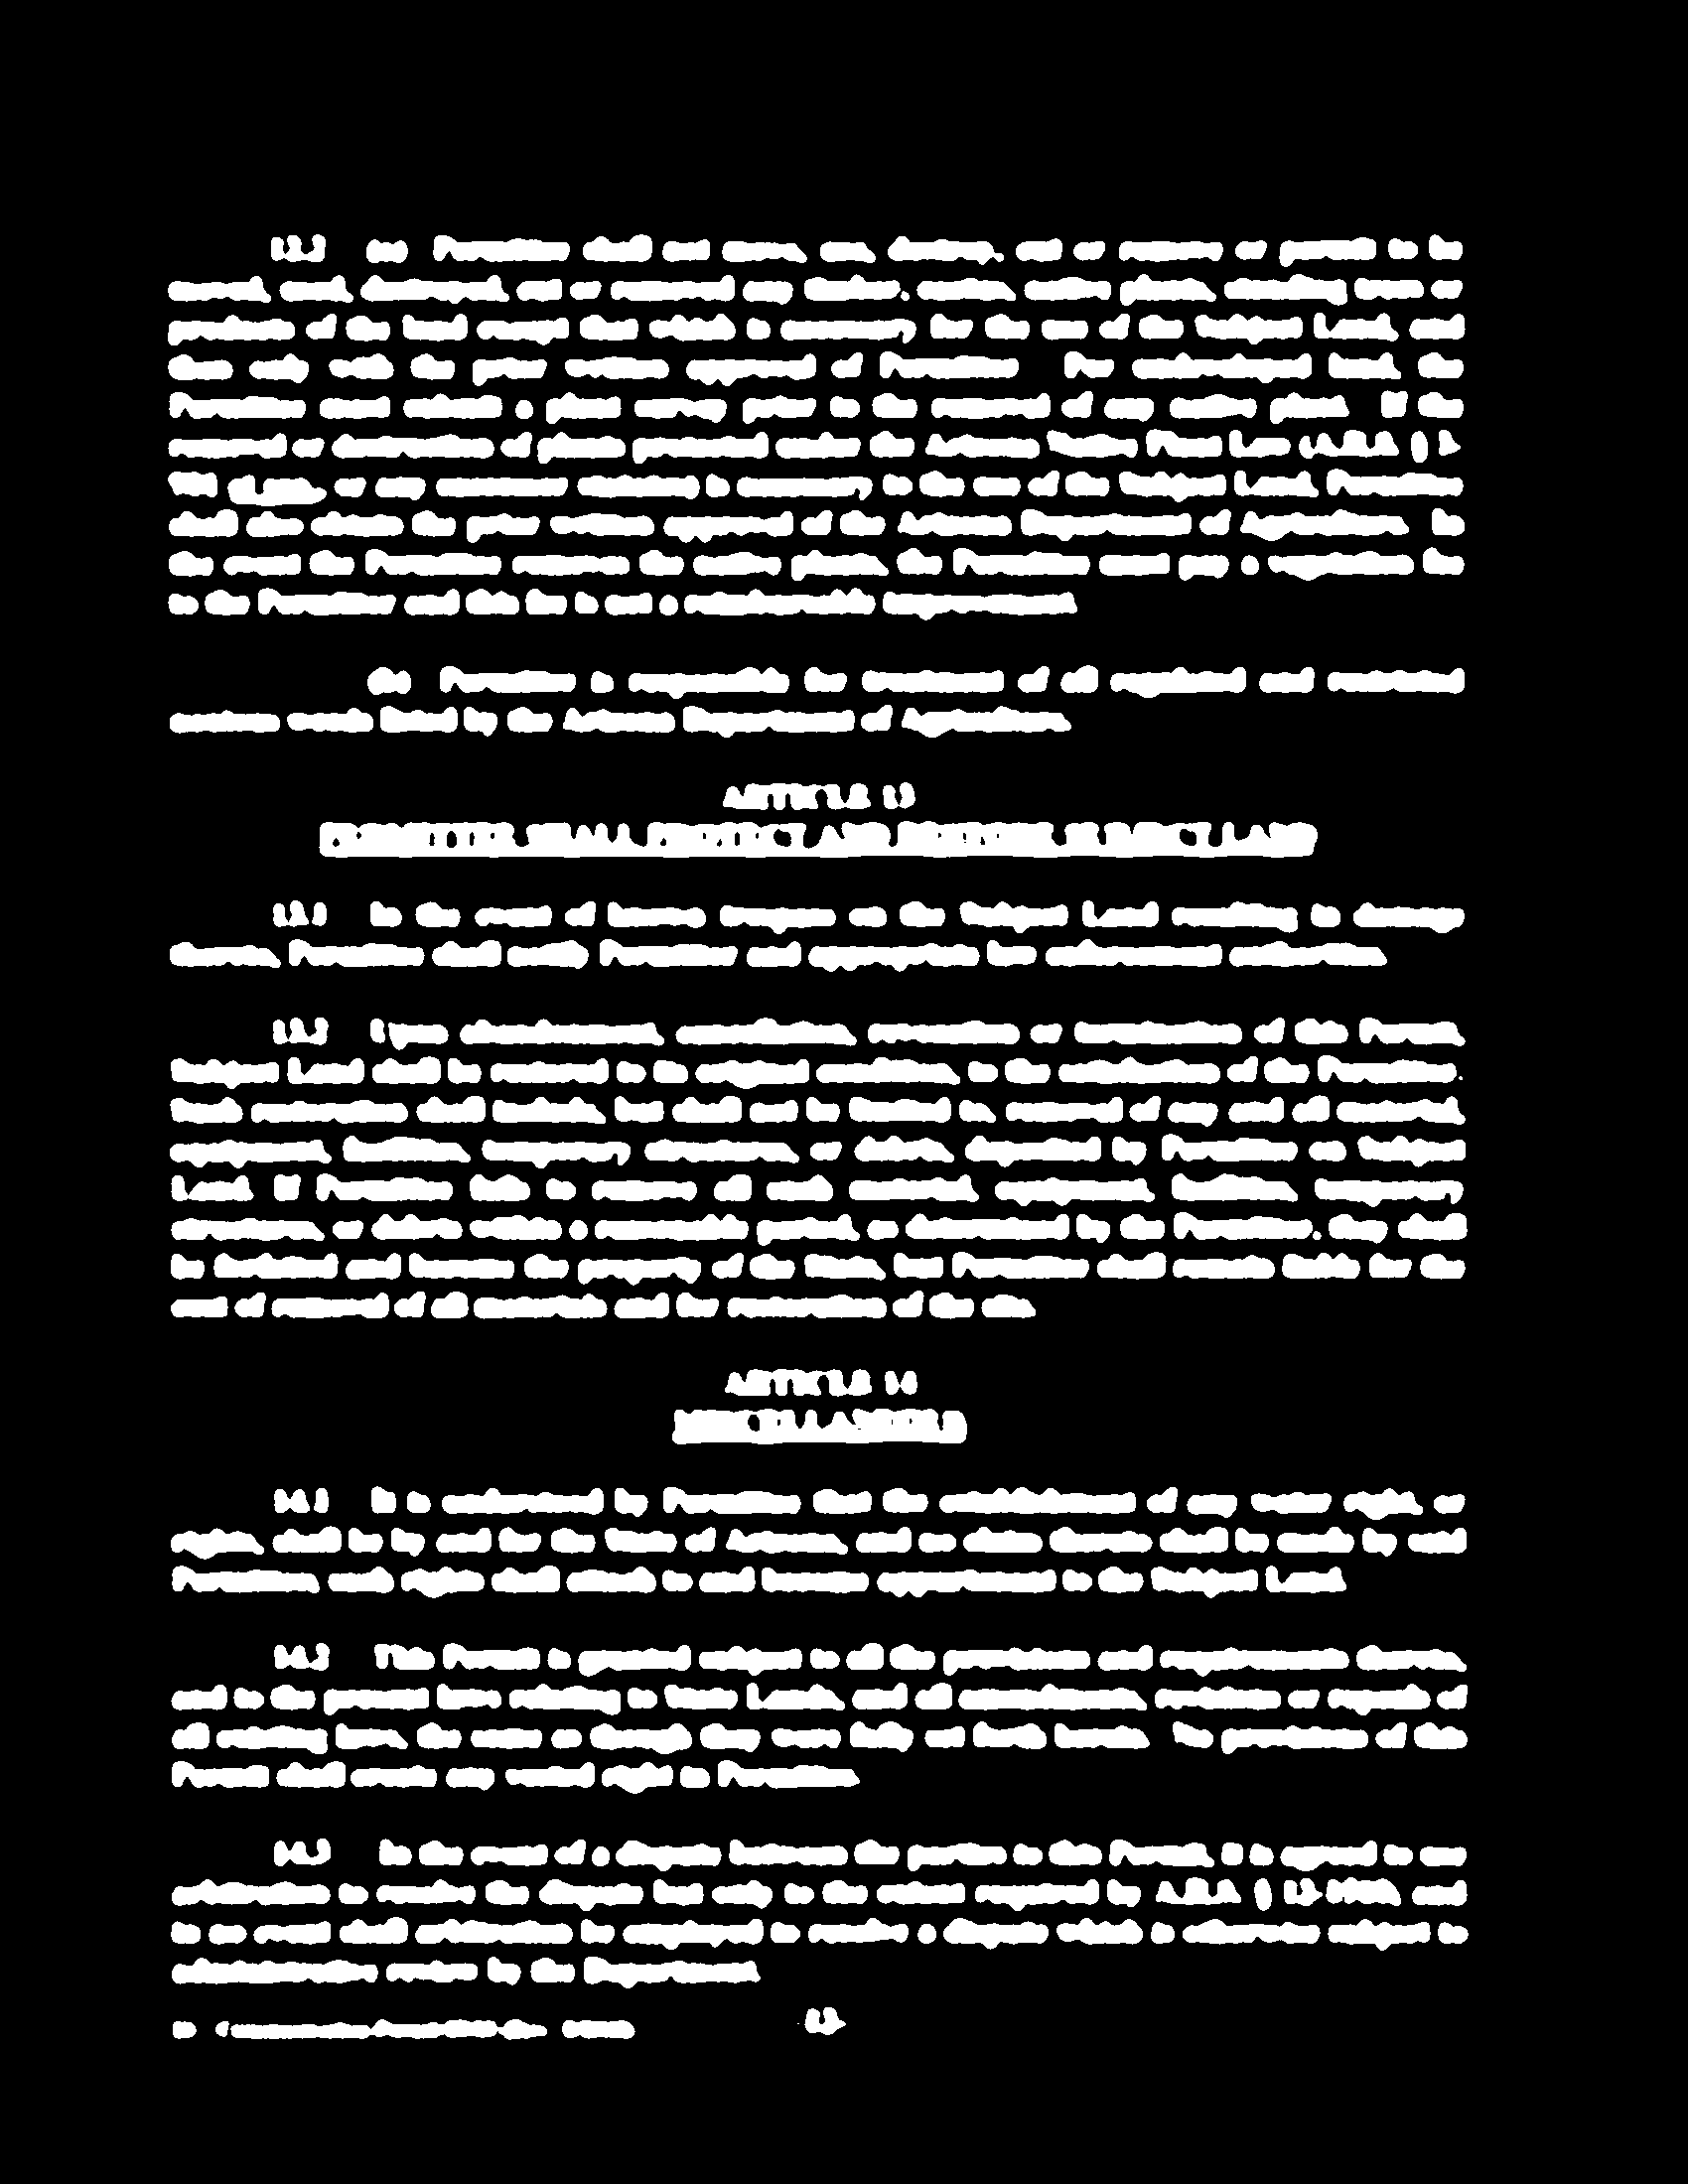
\includegraphics[scale=0.2]{img/paragraph/thresh.png}
    \caption{Бинаризованное изображение}
    \label{segmentation_threshold}
\end{figure}

Теперь необходимо найти и скорректировать все абзацы. Для этого найдем все контуры изображения с помощью метода из библиотеки $OpenCV$ \cite{opencv_contours} и находящиеся рядом контуры объединим.
В результате получим абзацы, границы которых изображены на рисунке ~\ref{segmentation_output}.

\begin{figure}
    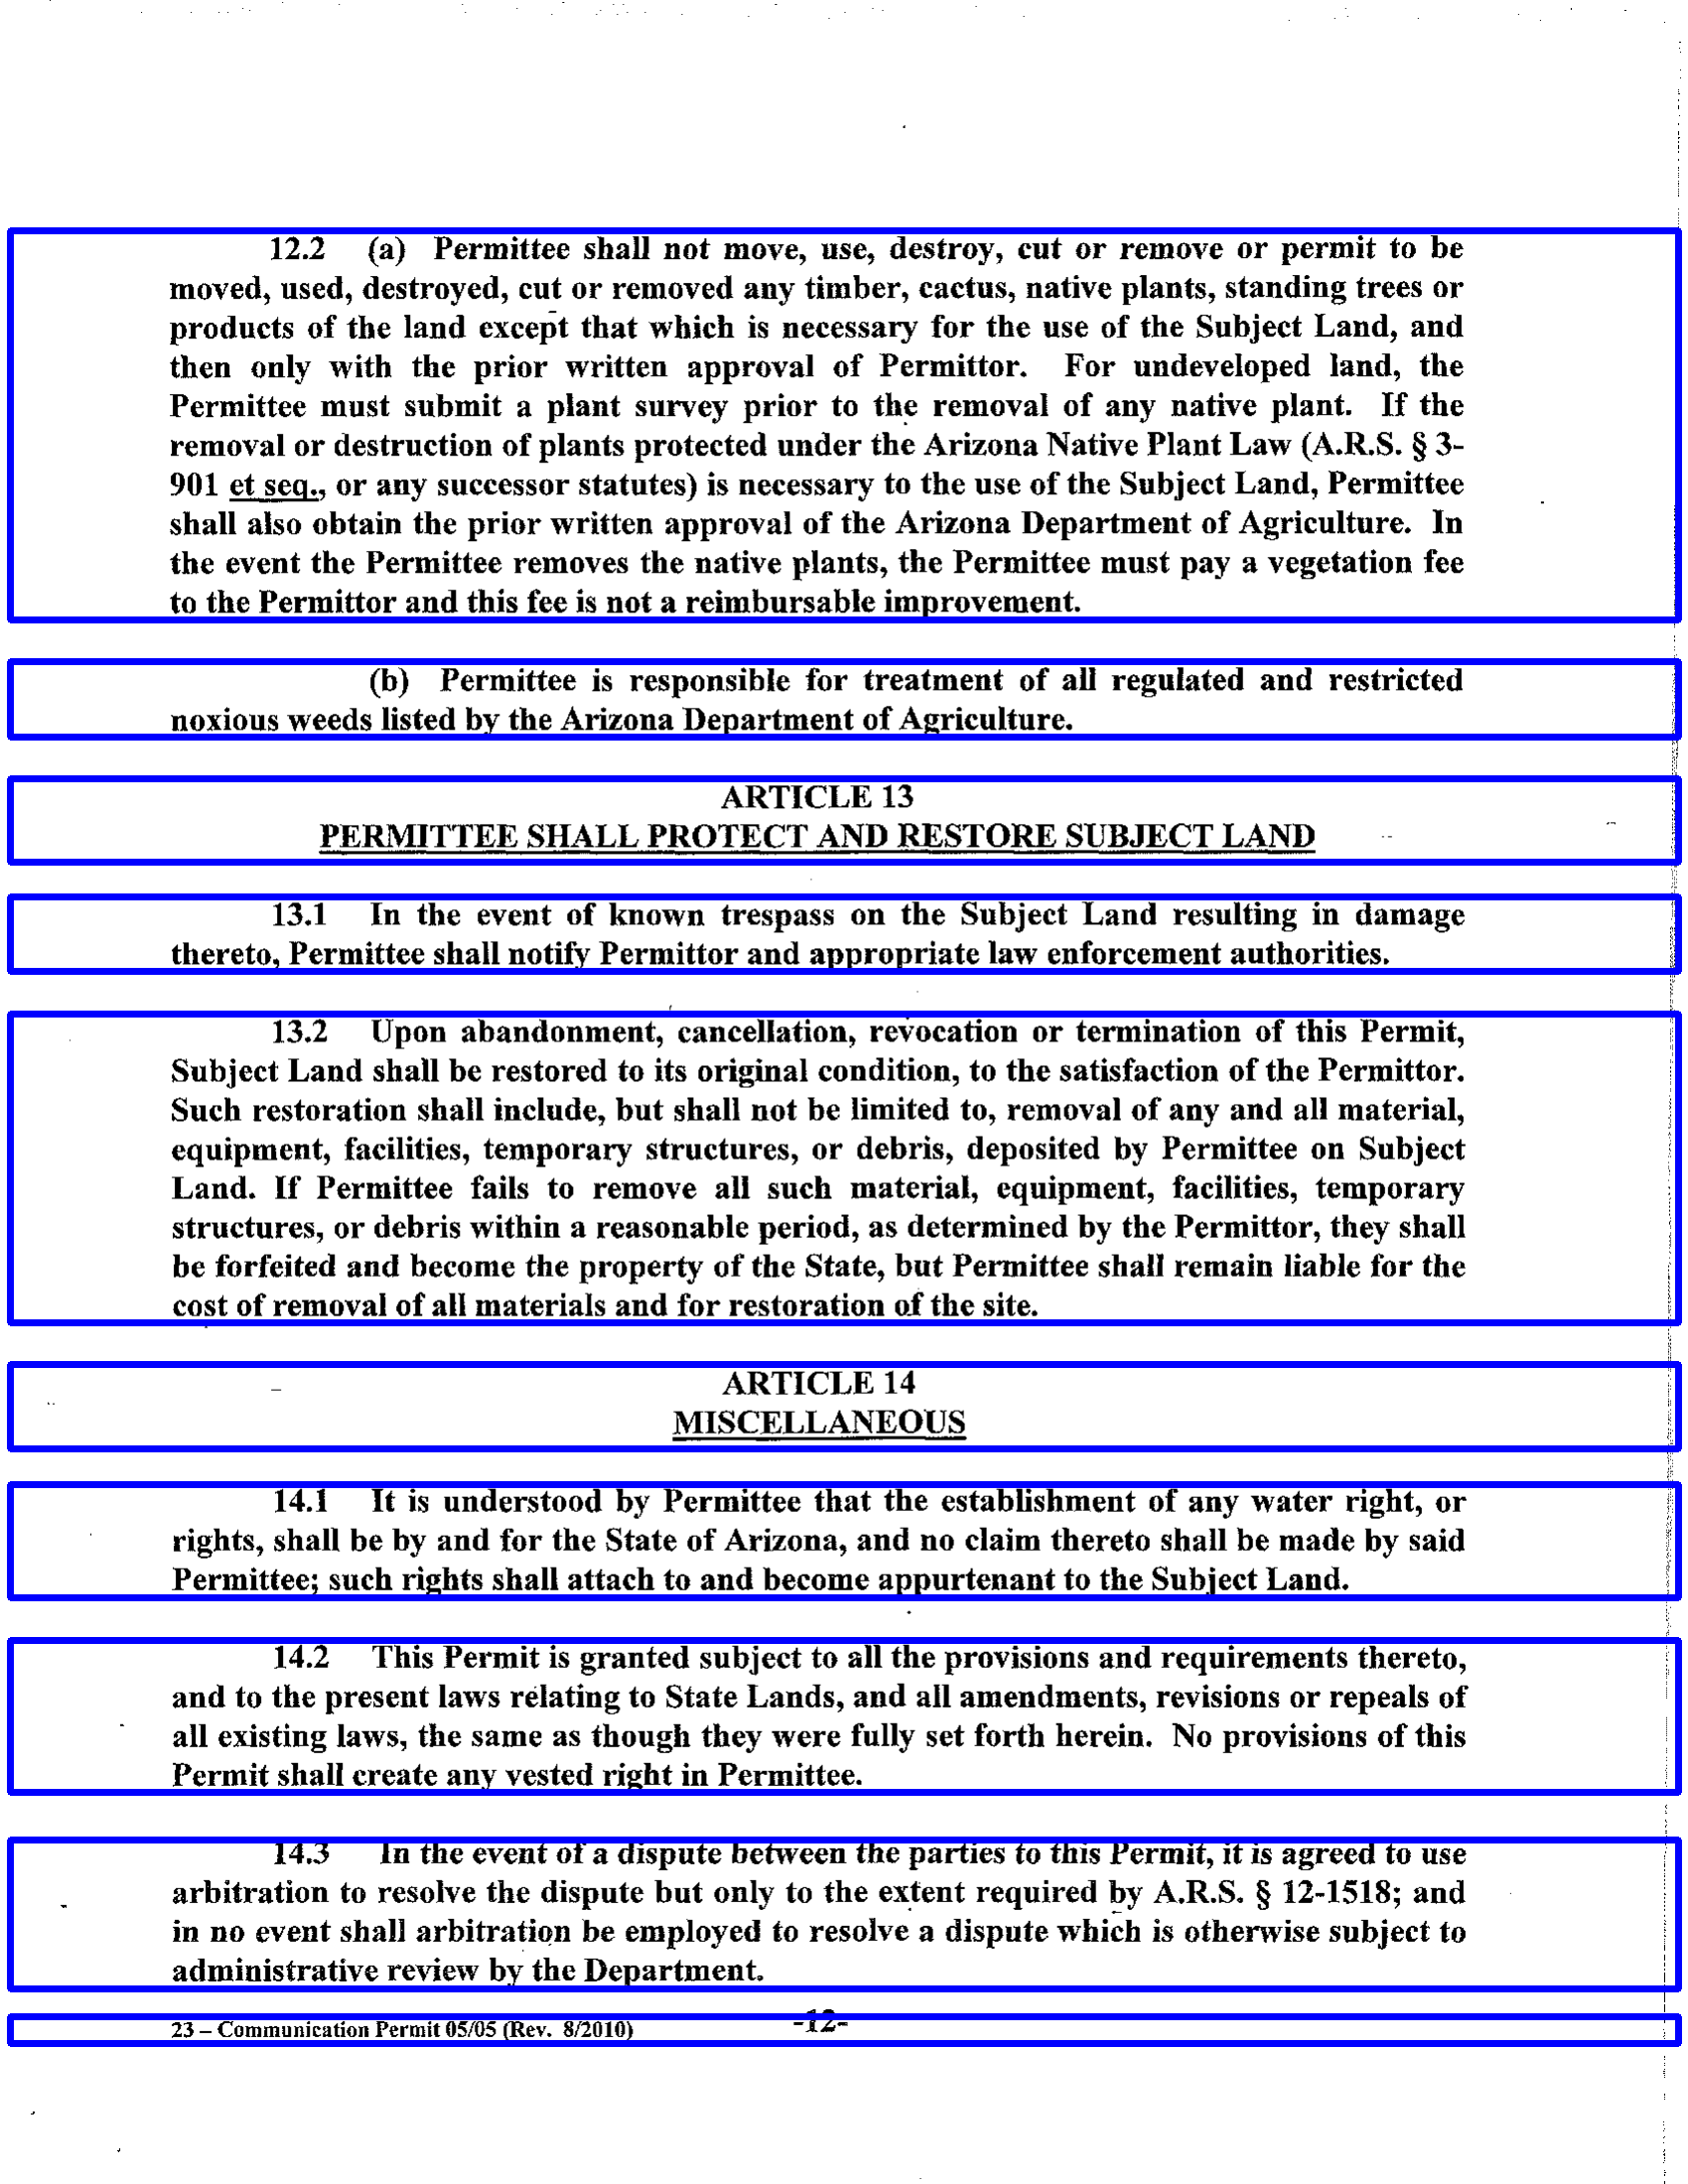
\includegraphics[scale=0.2]{img/paragraph/out.png}
    \caption{Найденные абзацы}
    \label{segmentation_output}
\end{figure}

\subsubsection{Сегментация $pdf$ файла}
В настоящее время файл формата $pdf$ широко распространен, и важно уметь обрабатывать данный формат, так как многие публикации и статьи хранятся именно в этом формате.

Существует несколько типов $pdf$ файлов, такие как:
\begin{itemize}
    \item \textbf{Программно генерируемые $pdf$ файлы}: эти $pdf$ создаются программно, например, предмет данной работы, \LaTeX\; можно преобразовать в $pdf$ файл. Данный тип файла может содержать различные компоненты, например, изображения, текст, ссылки.
    \item \textbf{Традиционные отсканированные документы}: такие $pdf$ файлы создаются из неэлектронных носителей, например, при сканировании. В данном случае $pdf$ выступает в роли контейнера для изображений. Поэтому с элементами на изображениях нельзя никак взаимодействовать.
\end{itemize}

В случае с отсканированными документами необходимо поступать как с изображением по описанному выше алгоритму. Однако, в случае с программно генерируемым файлом мы можем извлекать из него необходимую информацию, такую как: абзацы, изображения, таблицы и т.д.
На данном этапе нас интересует извлечение абзацев. Для задачи парсинга $pdf$ файла использовалась библиотека $PyMuPDF$ \cite{PyMuPDF}. С помощью этой библиотеки можно легко извлекать абзацы текста. На рисунке ~\ref{segmentation_pdf_input} представлен пример одной из страниц $pdf$ файла. На рисунке ~\ref{segmentation_pdf_output} представлены результаты сегментации на абзацы средствами библиотеки.
\begin{figure}
    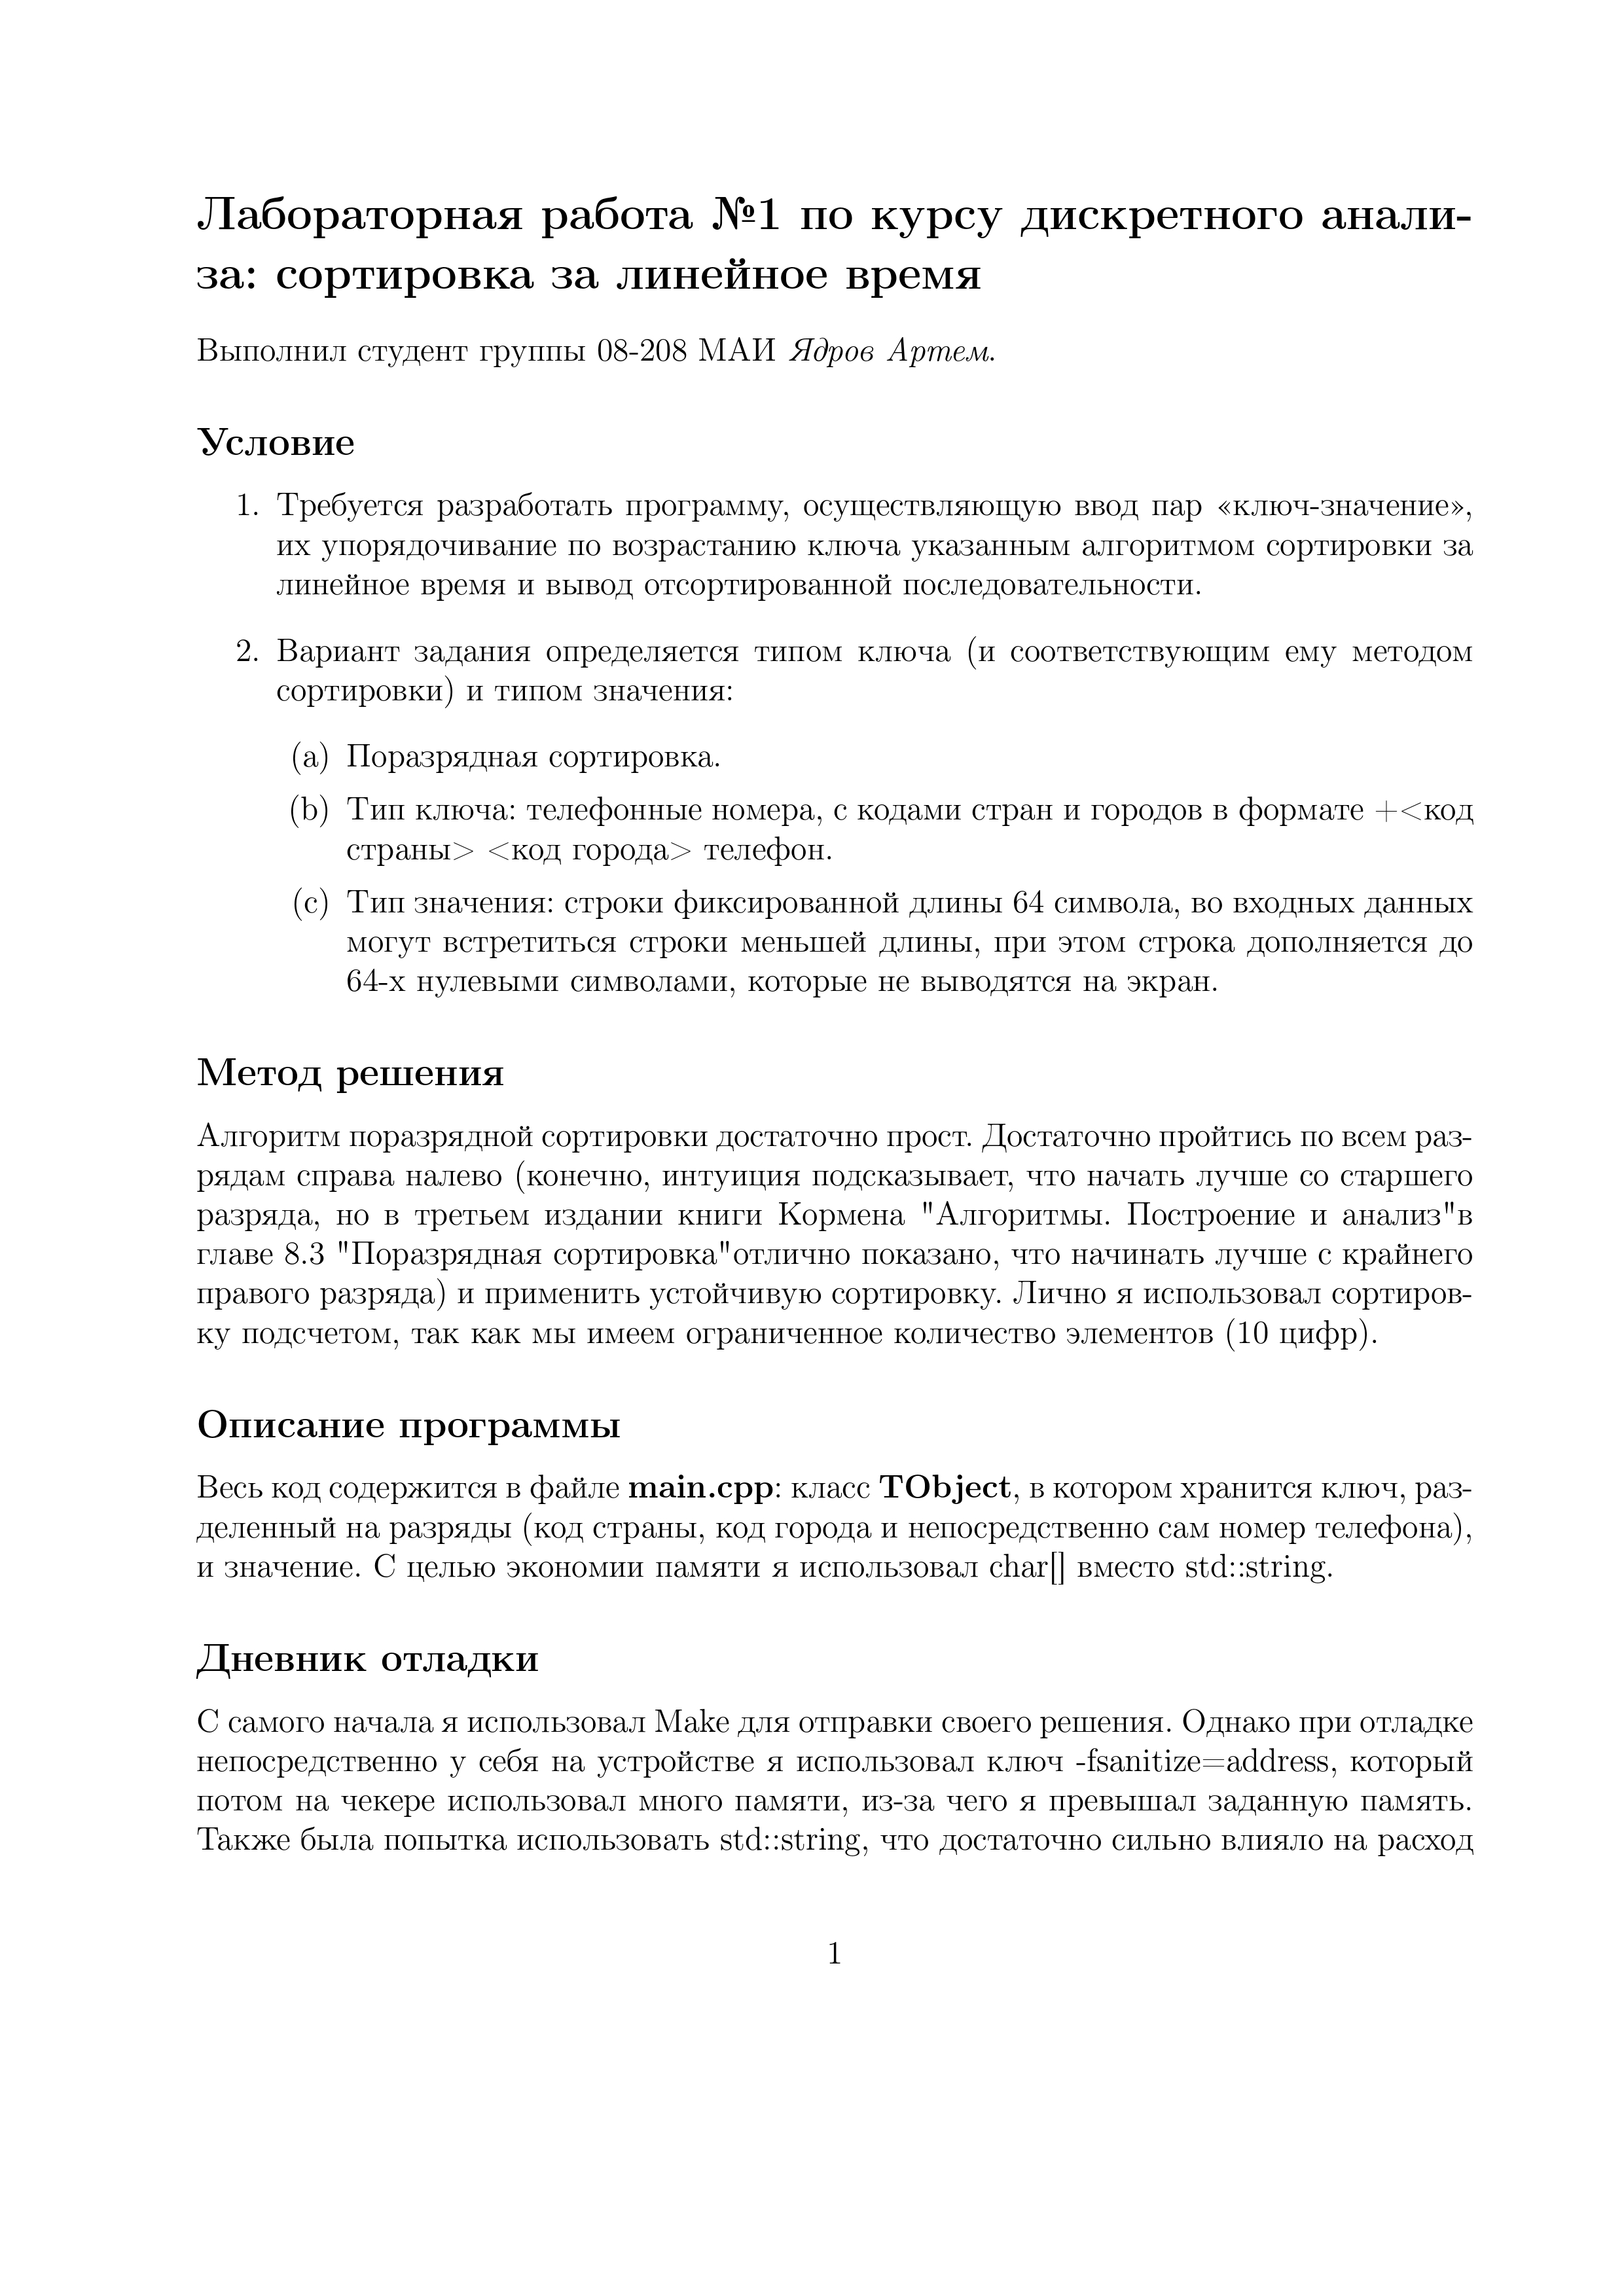
\includegraphics[scale=0.65]{img/paragraph/pdf_input.jpg}
    \caption{Пример страницы $pdf$}
    \label{segmentation_pdf_input}
\end{figure}

\begin{figure}
    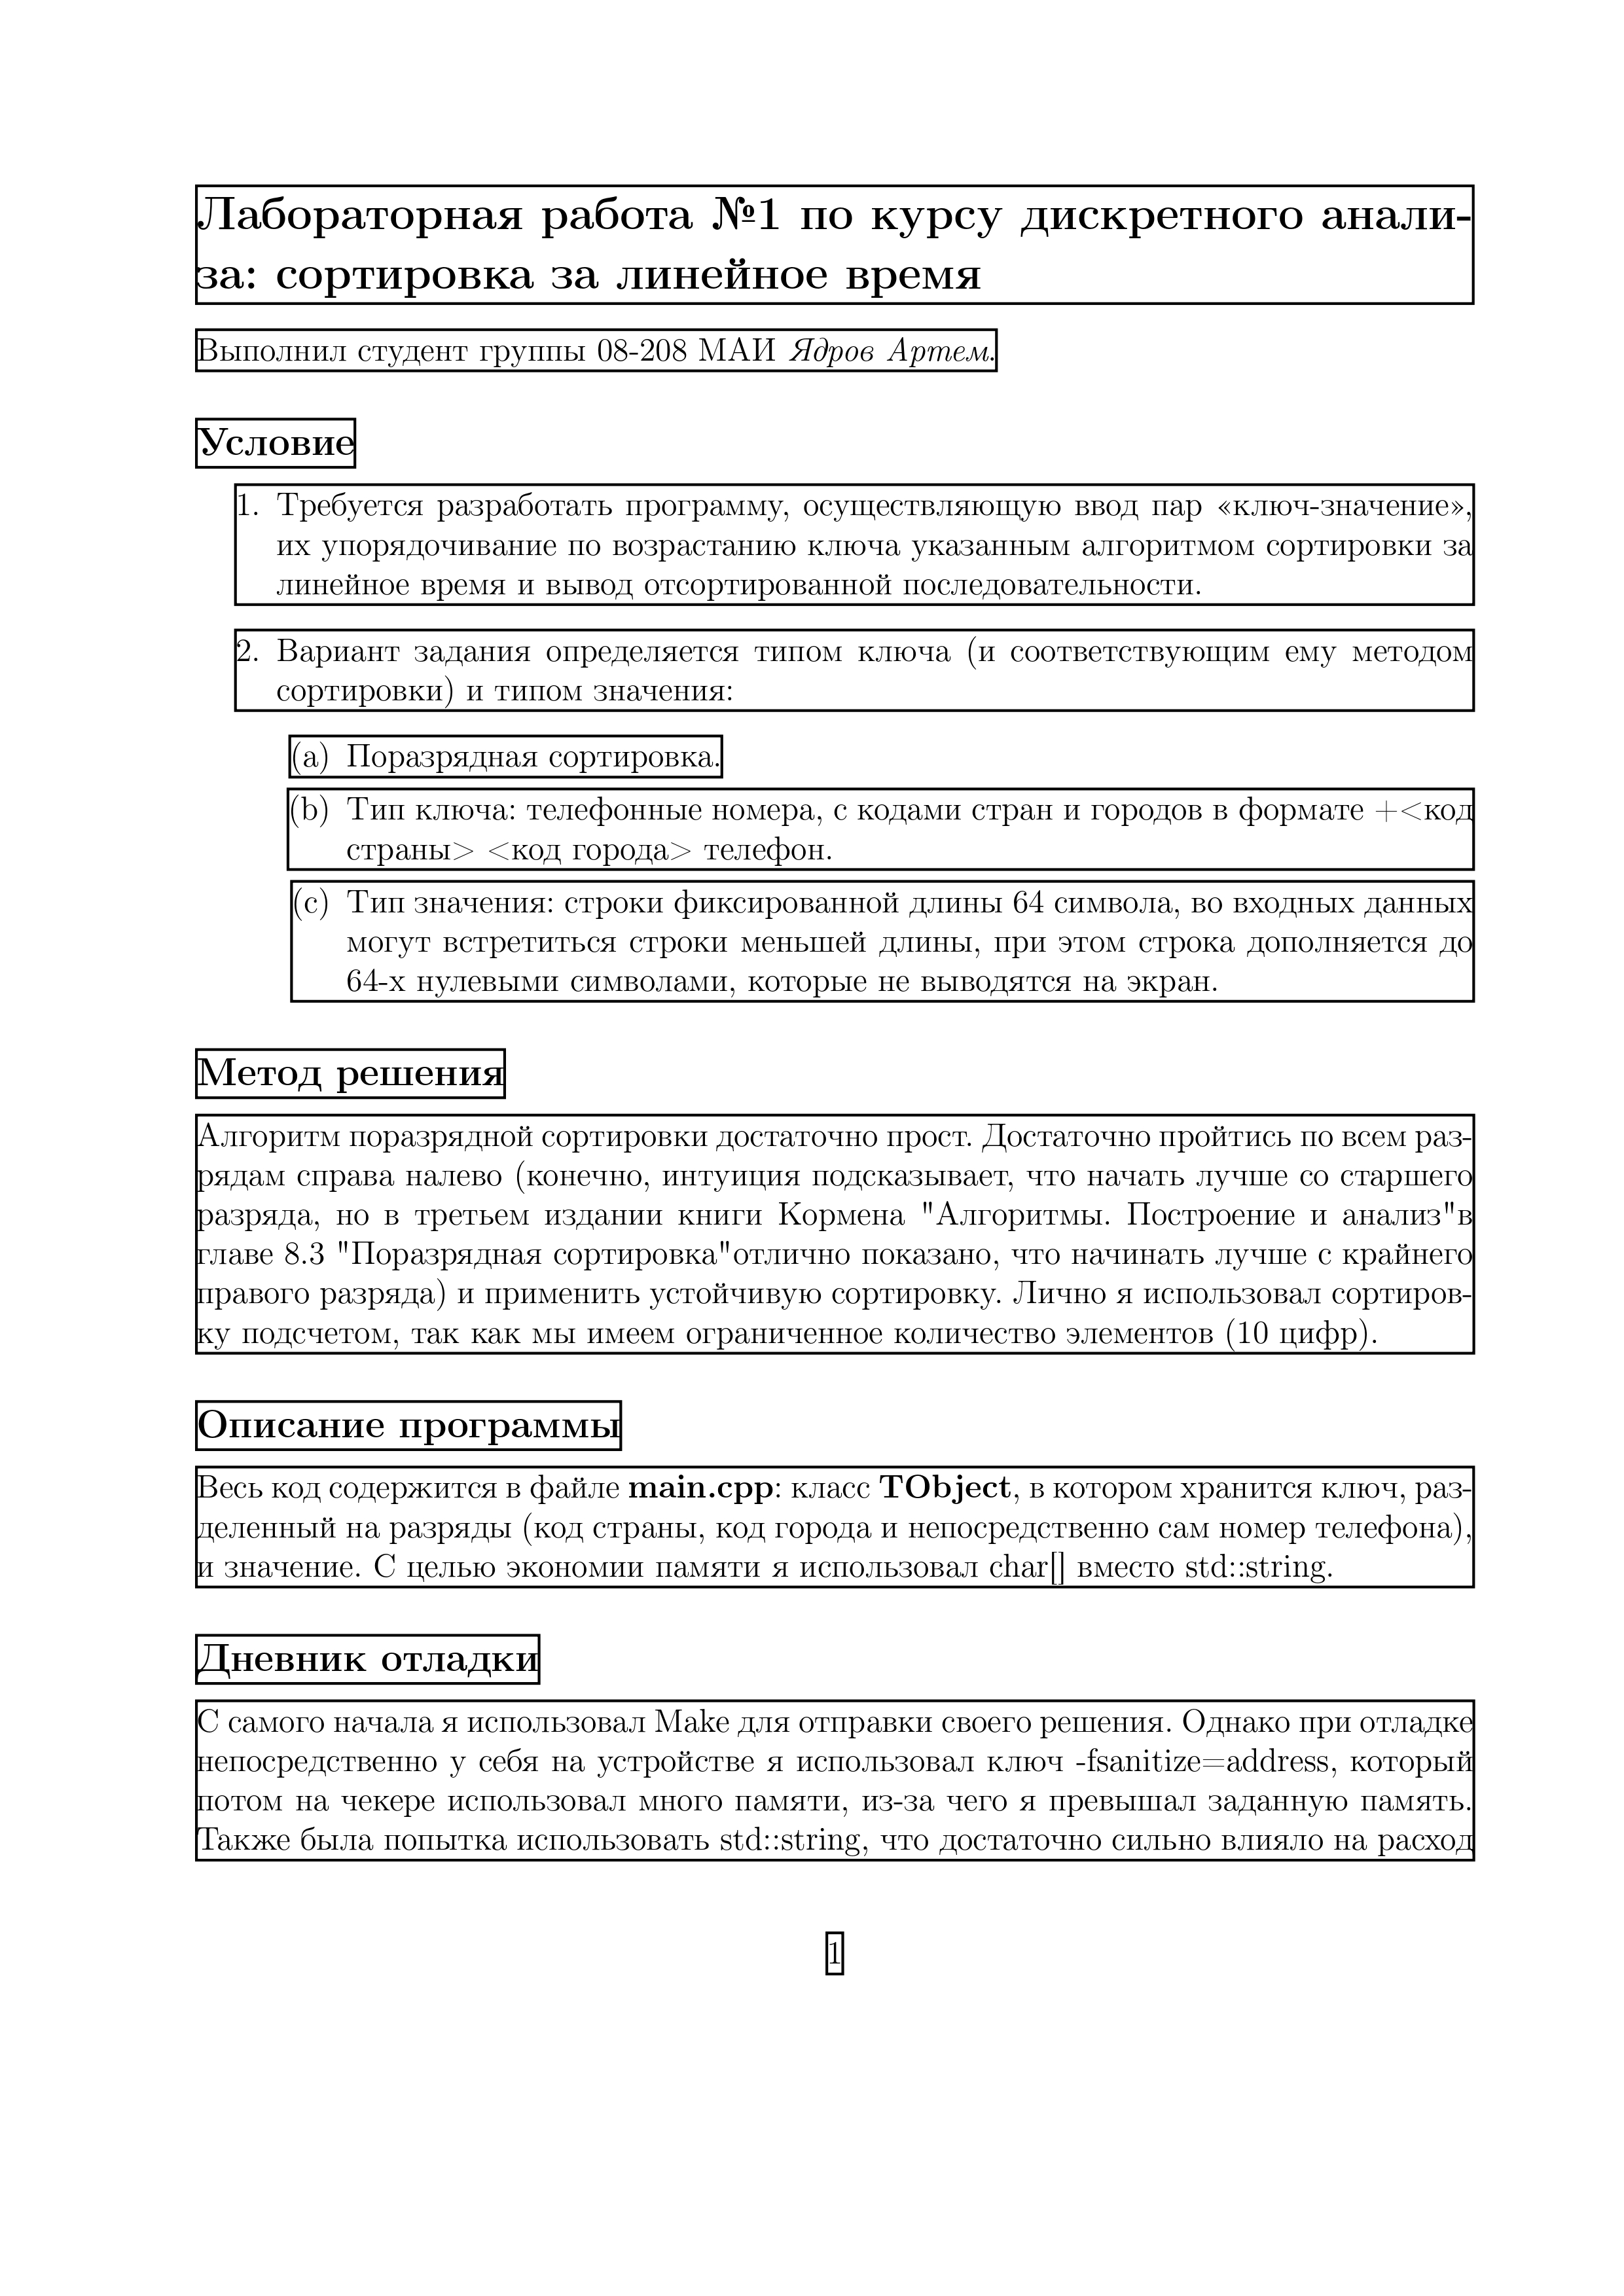
\includegraphics[scale=0.65]{img/paragraph/pdf_output.jpg}
    \caption{Пример страницы $pdf$ с размеченными абзацами}
    \label{segmentation_pdf_output}
\end{figure}

Мы можем наблюдать четко выделенные абзацы. Для сравнения к этому же изображению применим алгоритм сегментации изображения, описанный выше. 
На рисунке ~\ref{img_segmentation_output_pdf} показан результат применения этого алгоритма к изображению на рисунке ~\ref{segmentation_pdf_input}.

\begin{figure}
    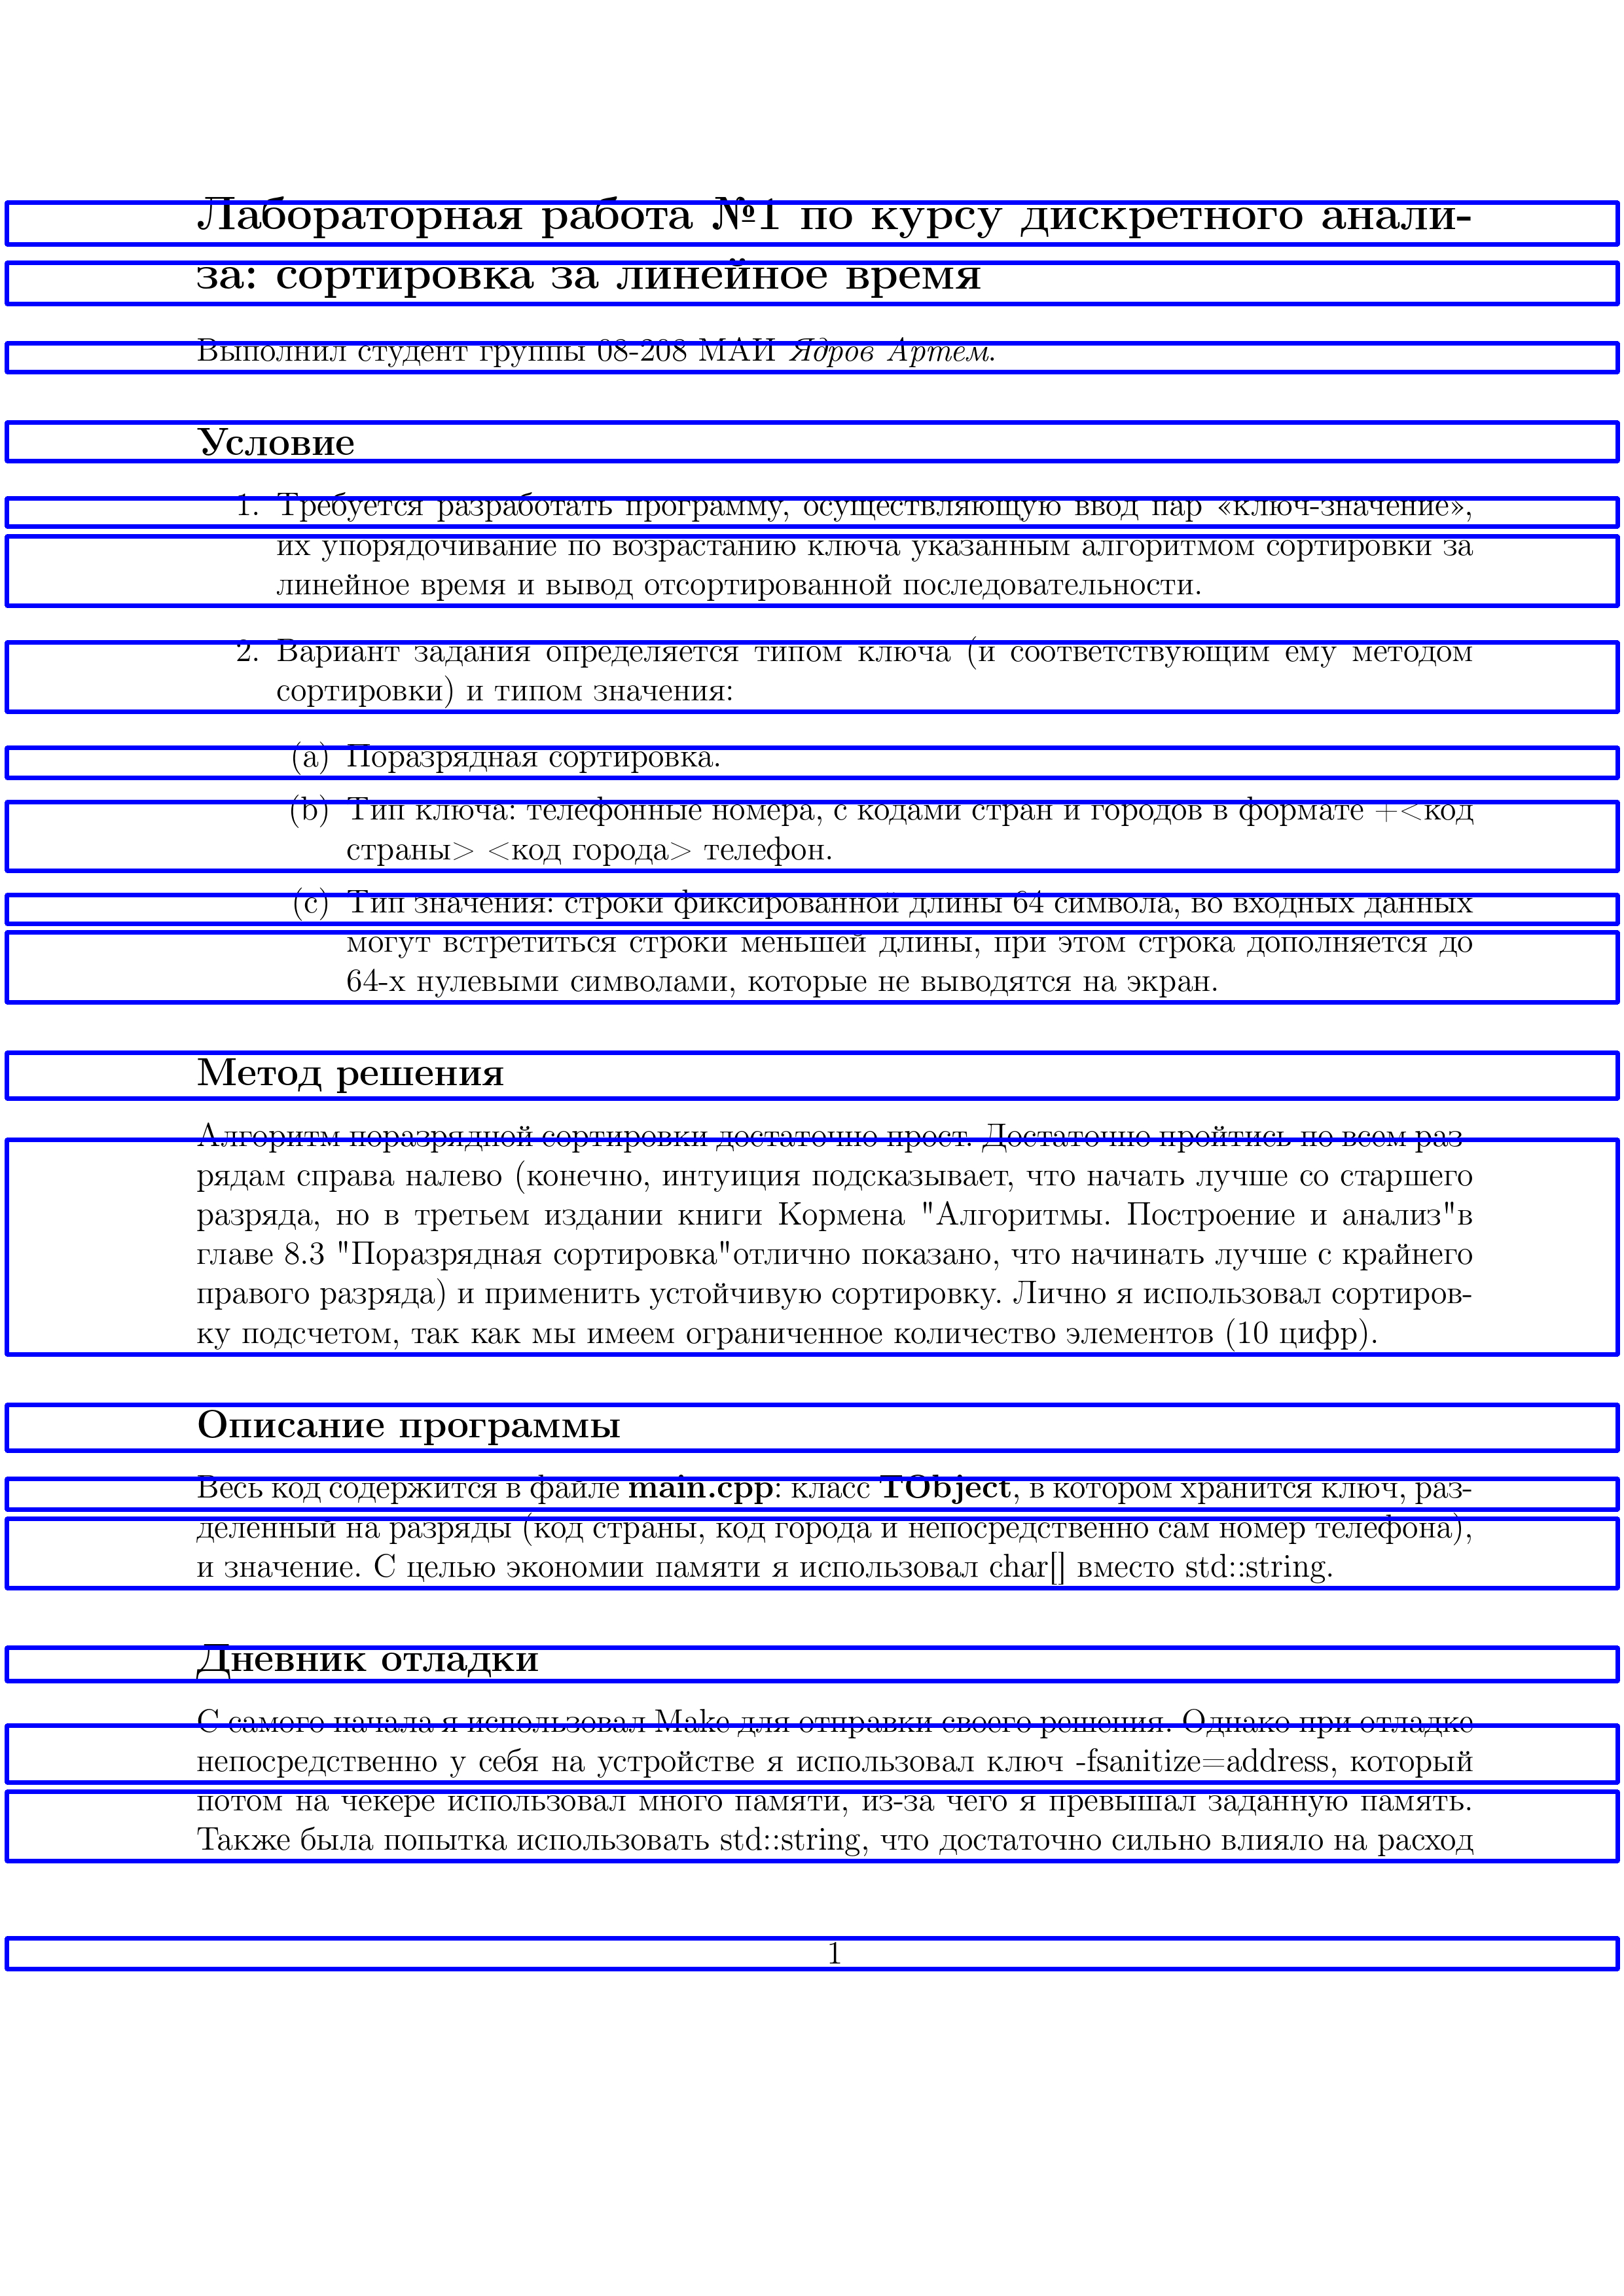
\includegraphics[scale=0.15]{img/paragraph/pdf_like_img_output.png}
    \caption{Пример страницы $pdf$ с размеченными абзацами алгоритмом сегментации изображения}
    \label{img_segmentation_output_pdf}
\end{figure}


\subsection{Выделение формул}
\subsubsection{Модель}

Для выделения формул недостаточно одних алгоритмов обработки изображений. Существует множество моделей, выполняющих распознавание объектов на изображении.
Одной из таких моделей является $YOLO$ \cite{yolo}. Данная модель обладает следующими преимуществами:
\begin{itemize}
    \item быстродействие: нейросеть работает в реальном времени, поэтому её используют для распознавания объектов на фото и видео <<здесь и сейчас>>;
    \item точность: нейросеть $YOLO$ умеет распознавать объекты разных размеров в пределах одного кадра;
    \item универсальность: нейросеть $YOLO$ способна определять как хорошо знакомые ей объекты, так и те, с которыми она ещё не сталкивалась;
    \item простота: модель $YOLO$ можно запросто запускать и дообучать с помощью $Tensorflow$ \cite{tensorflow}.
\end{itemize}

Однако, данная модель не специализирована на какой-то одной задаче, поэтому будет проигрывать специализированным моделям.

На основании плюсов данной модели, а также на основании самой архитектуры системы, позволяющую при необходимости легко заменить выбранную модель на другую, было принято решение использовать для распознования формул модель $YOLO$ последней версии $v8$.

\subsubsection{Данные для обучения}

В качестве данных для обучения был взят датасет $ICDAR-2021$ ($International\;Conference\;on\;Document\;Analysis\;and\;Recognition$). Он содержит набор изображений текстовых документов, содержащих формулы, 
а также для каждого изображения имеется набор координат ограничивающих рамок ($"bounding\; boxes"$) для каждой формулы.
Размер датасета составляет 5171 изображений.
На рисунках ~\ref{dataset_input} и ~\ref{dataset_output} показаны примеры входного изображения и изображения с метками формул соответственно.

\begin{figure}
    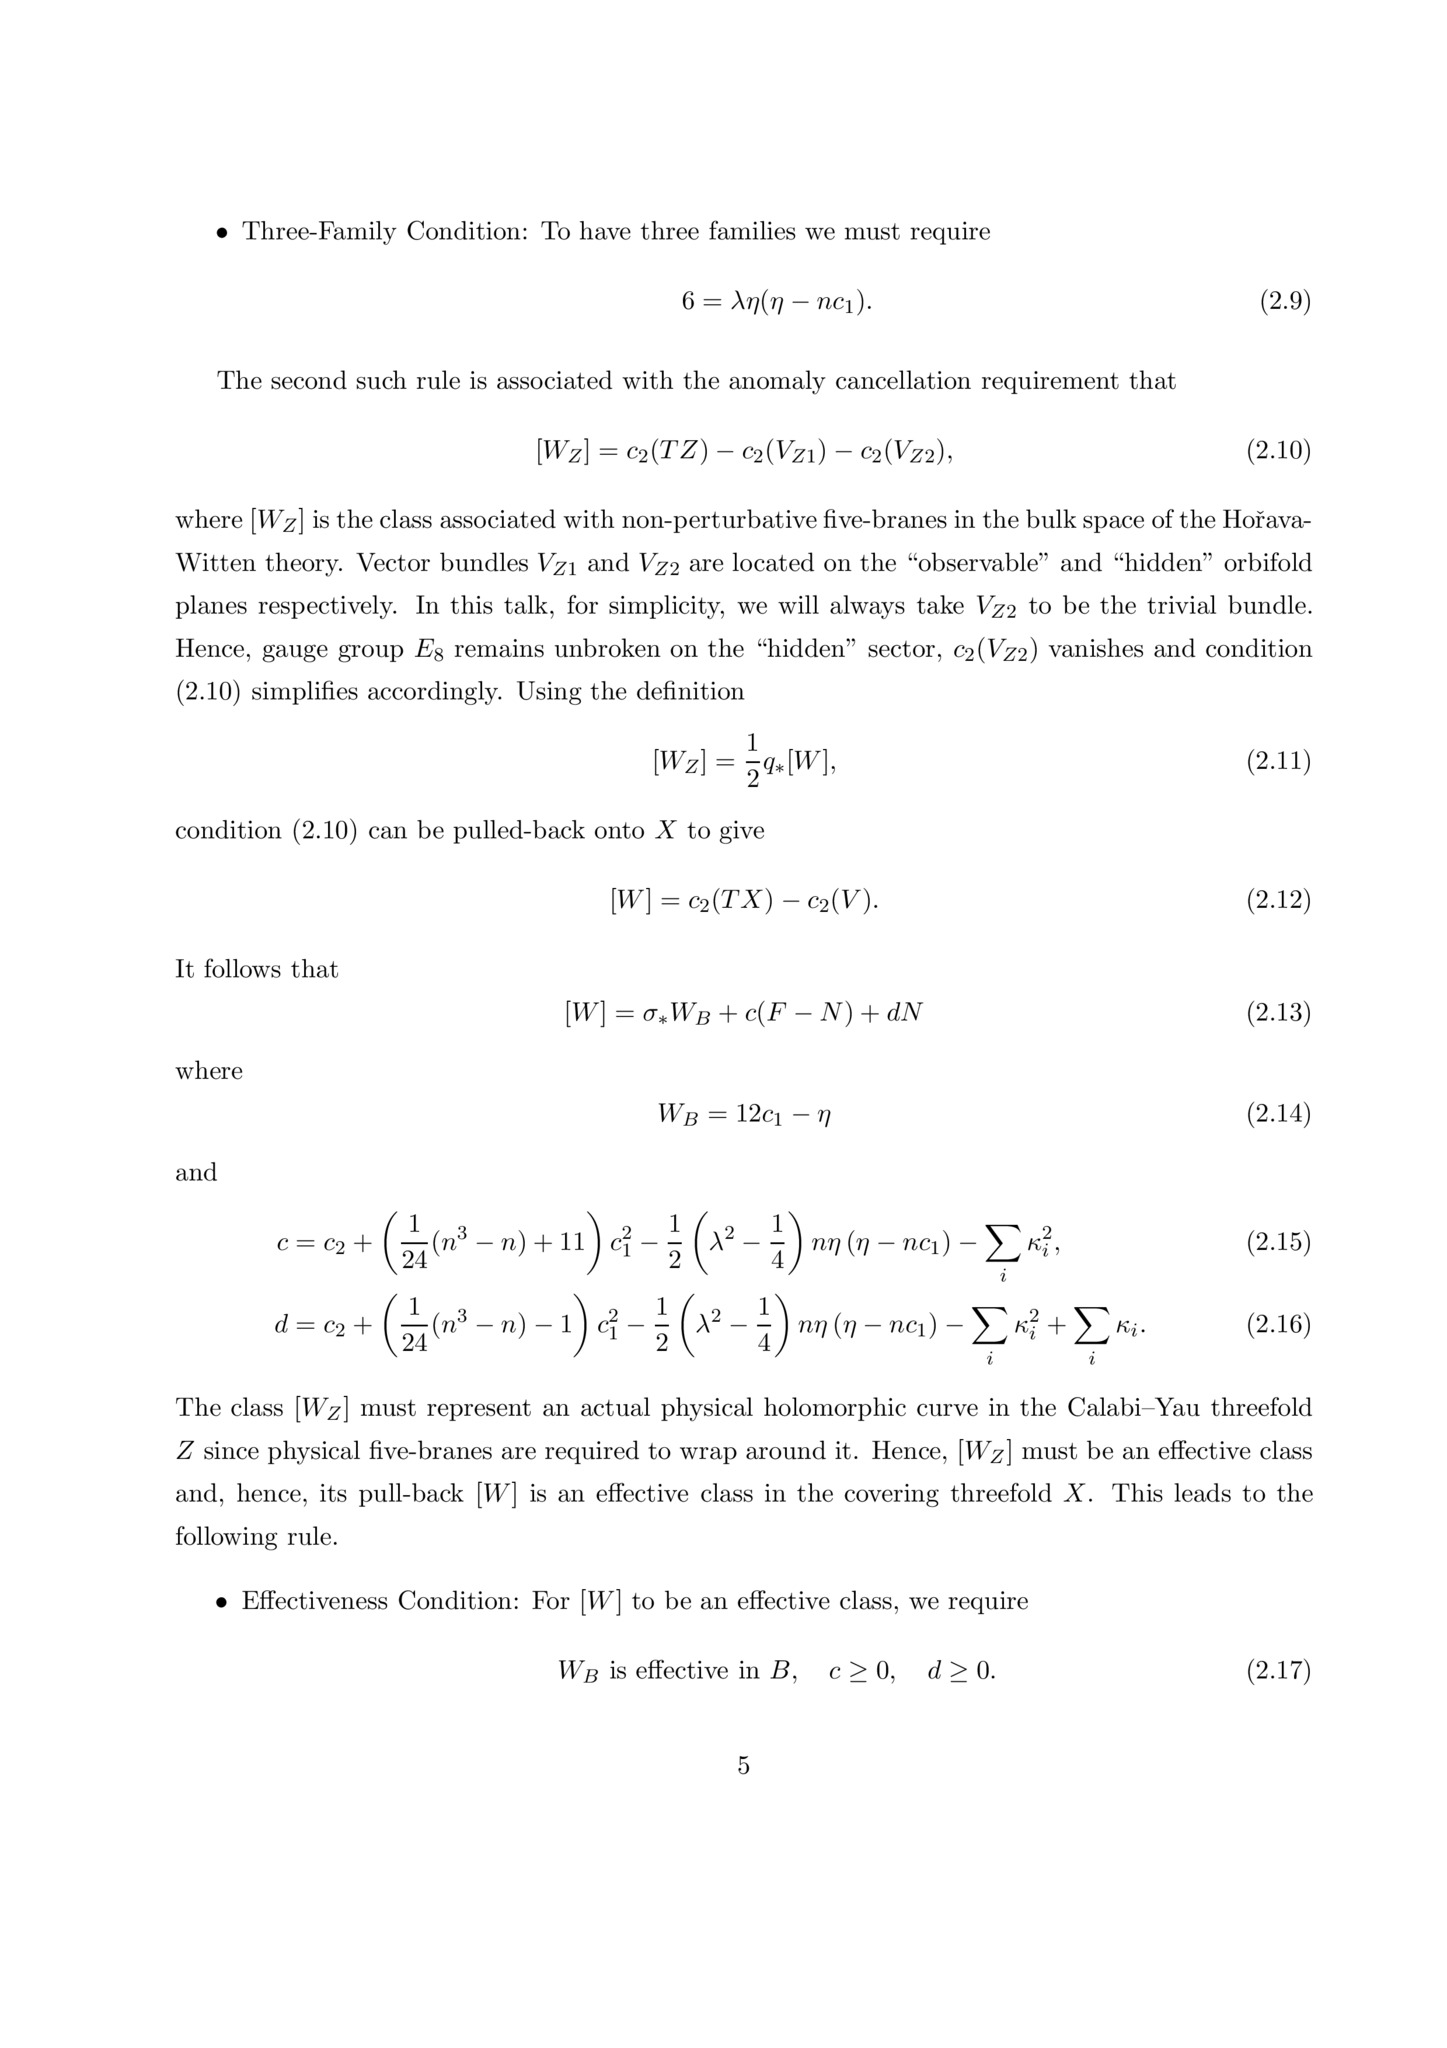
\includegraphics[scale=0.25]{img/dataset/input.jpg}
    \caption{Пример входного изображения}
    \label{dataset_input}
\end{figure}

\begin{figure}
    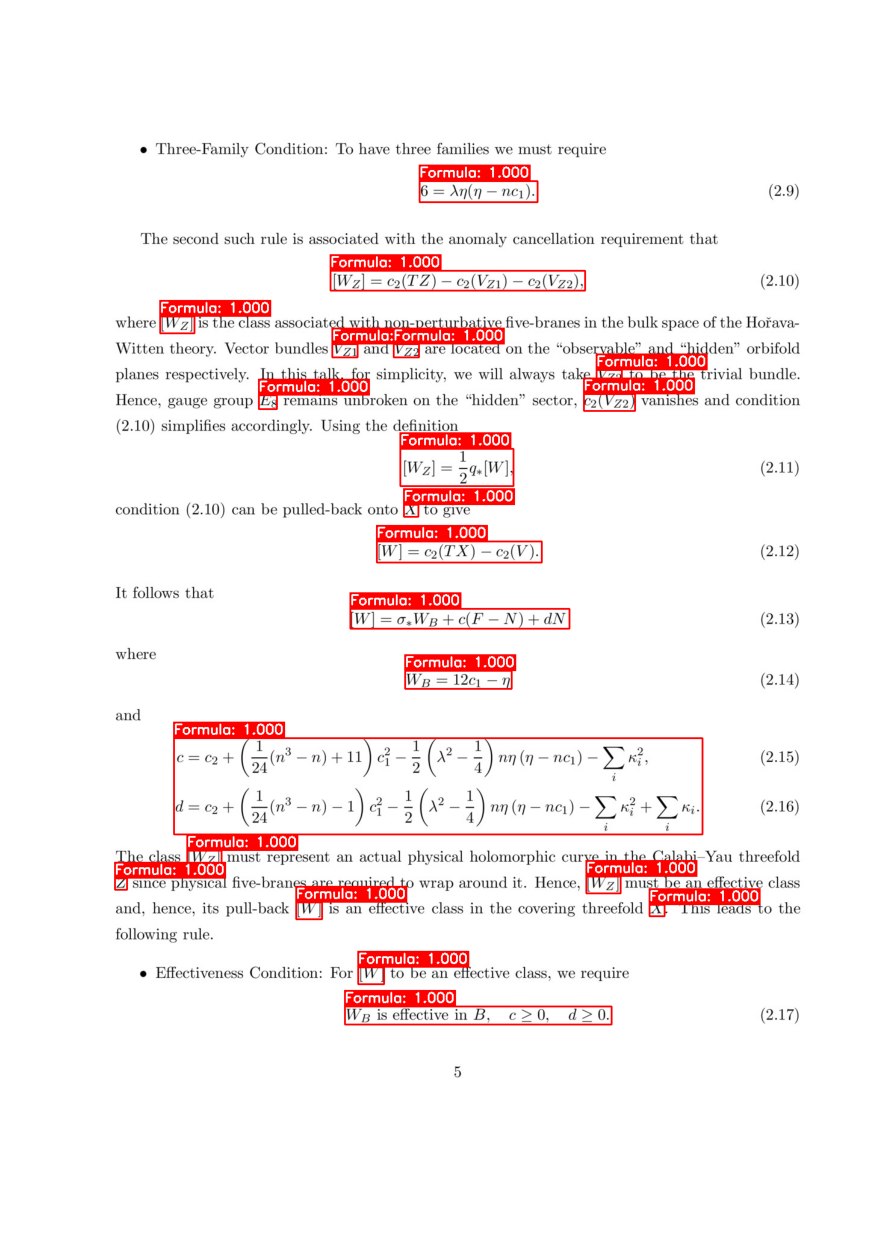
\includegraphics[scale=0.5]{img/dataset/parsed.png}
    \caption{Пример изображения с метками формул}
    \label{dataset_output}
\end{figure}

\subsubsection{Обучение}

Обучение проводилось на платформе $Kaggle$ \cite{kaggle} с логгированием в системе $wandb$ \cite{wandb}. В качестве графического процессора использовались две видеокарты $Tesla\;T4$
После обучения модели мы переходим к оценки ее эффективности. Посмотрим на полученные с помощью $wandb$ графики описанных выше метрик.
\begin{figure}
    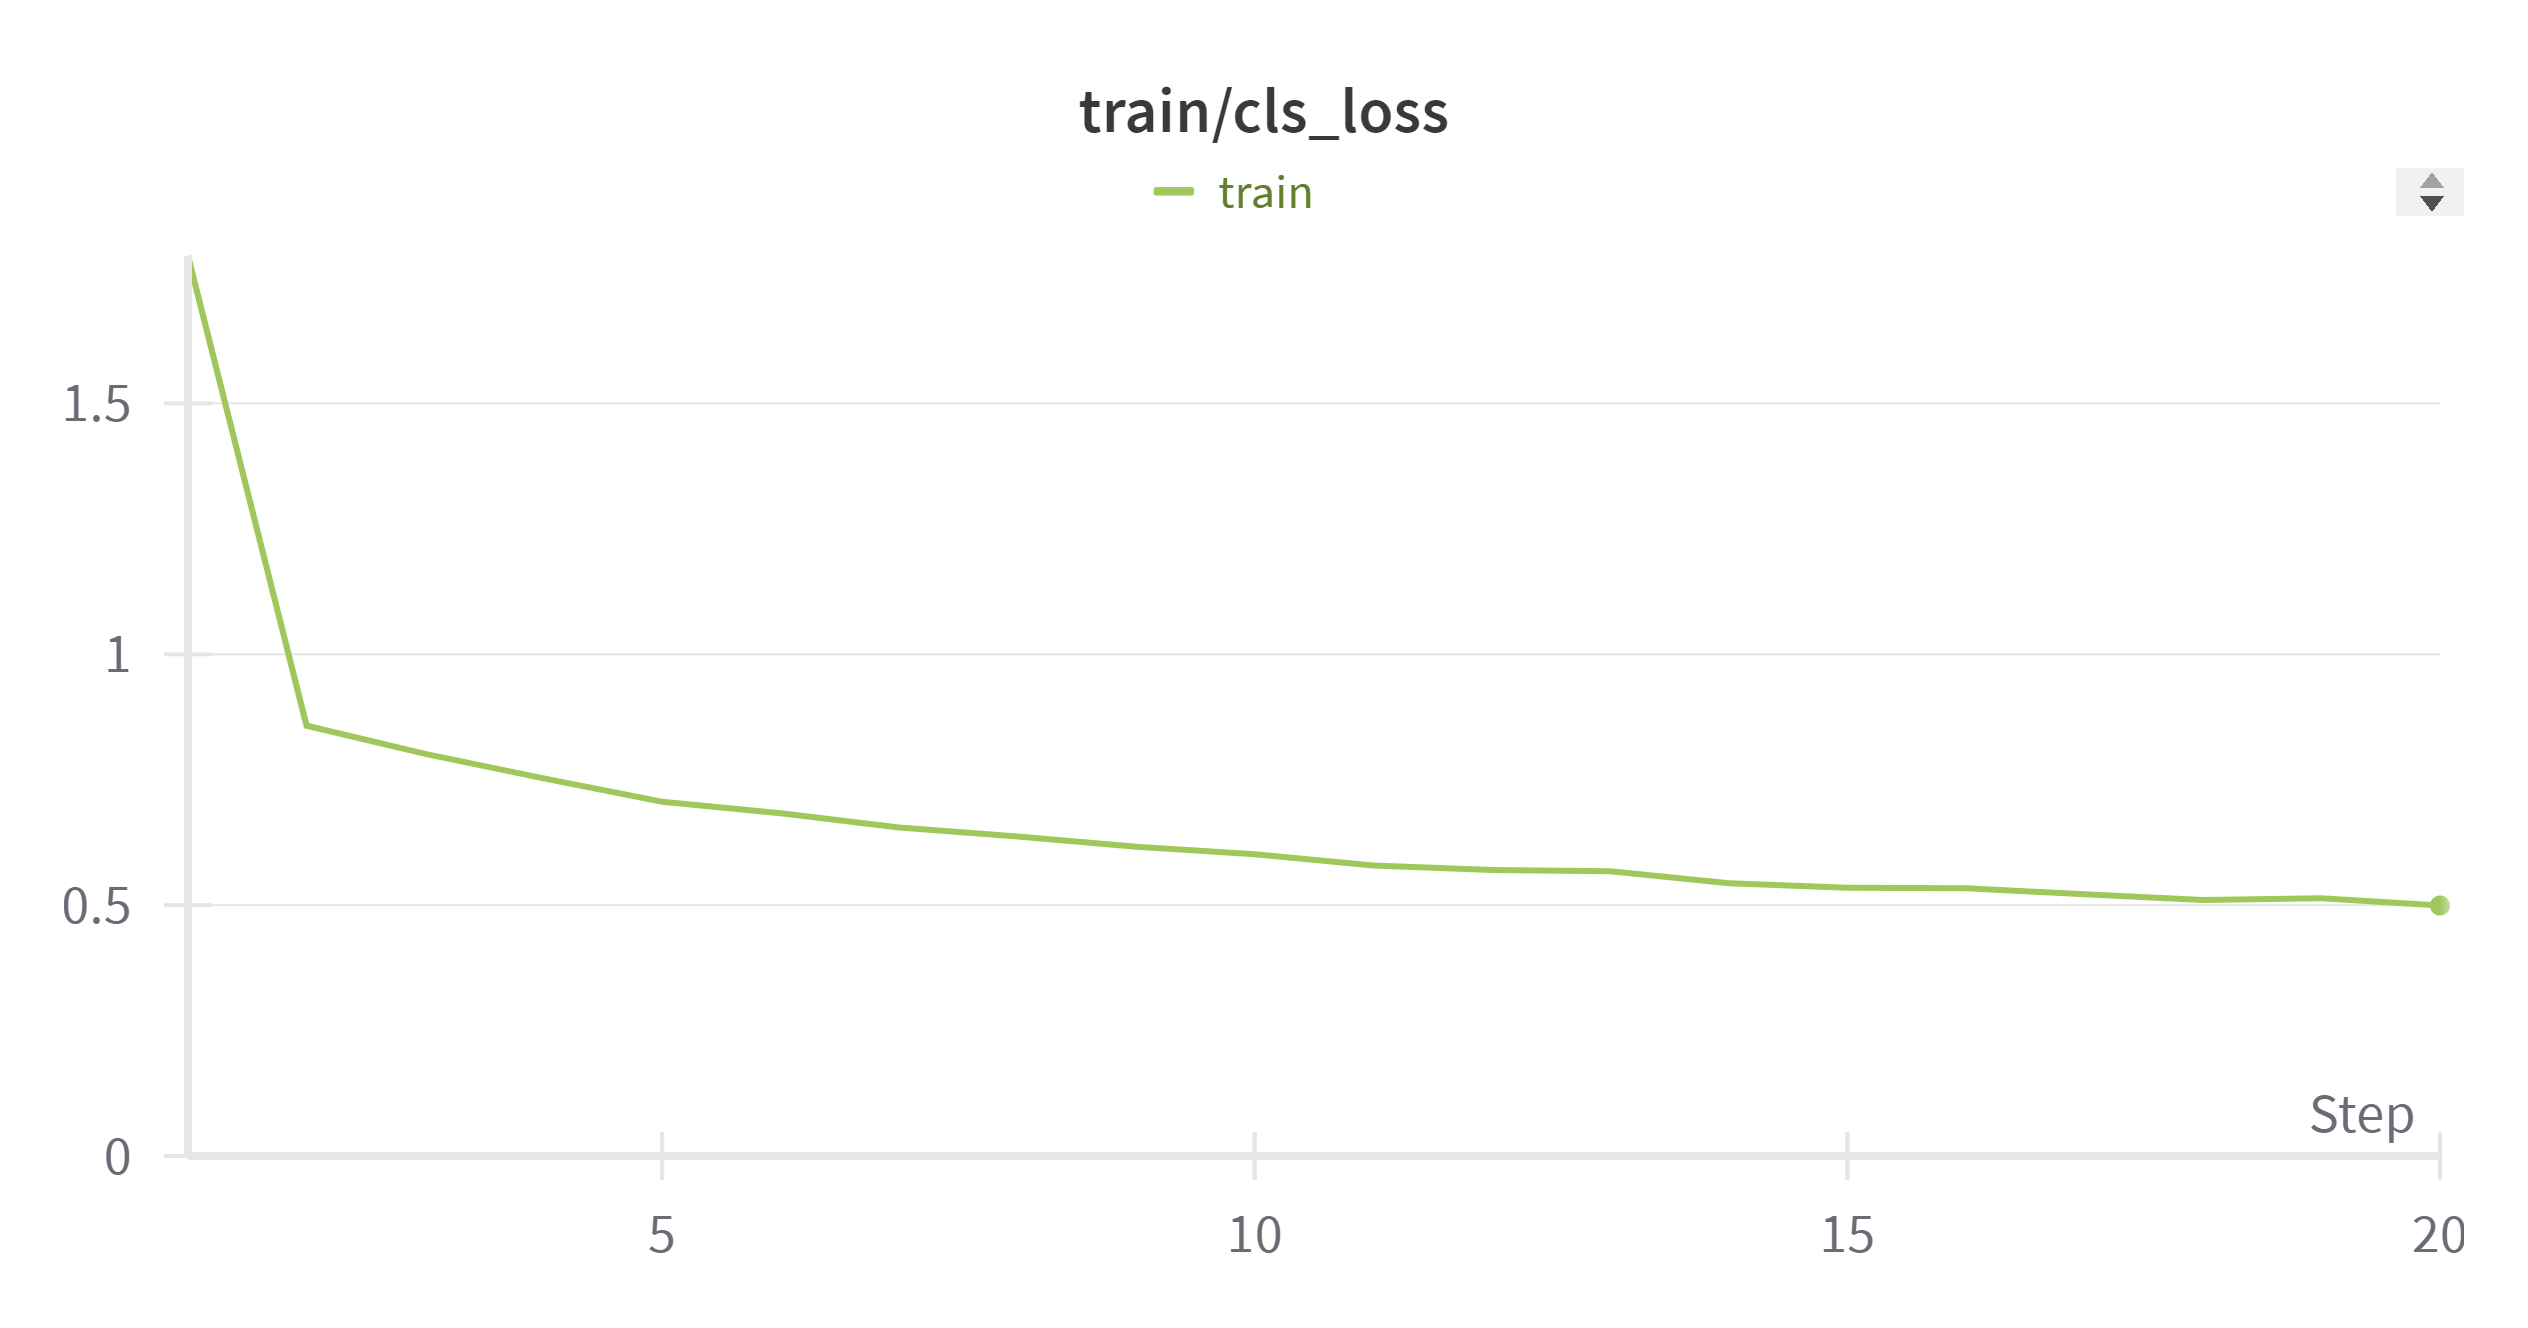
\includegraphics[scale=0.15]{img/train/train_cls_loss.png}
    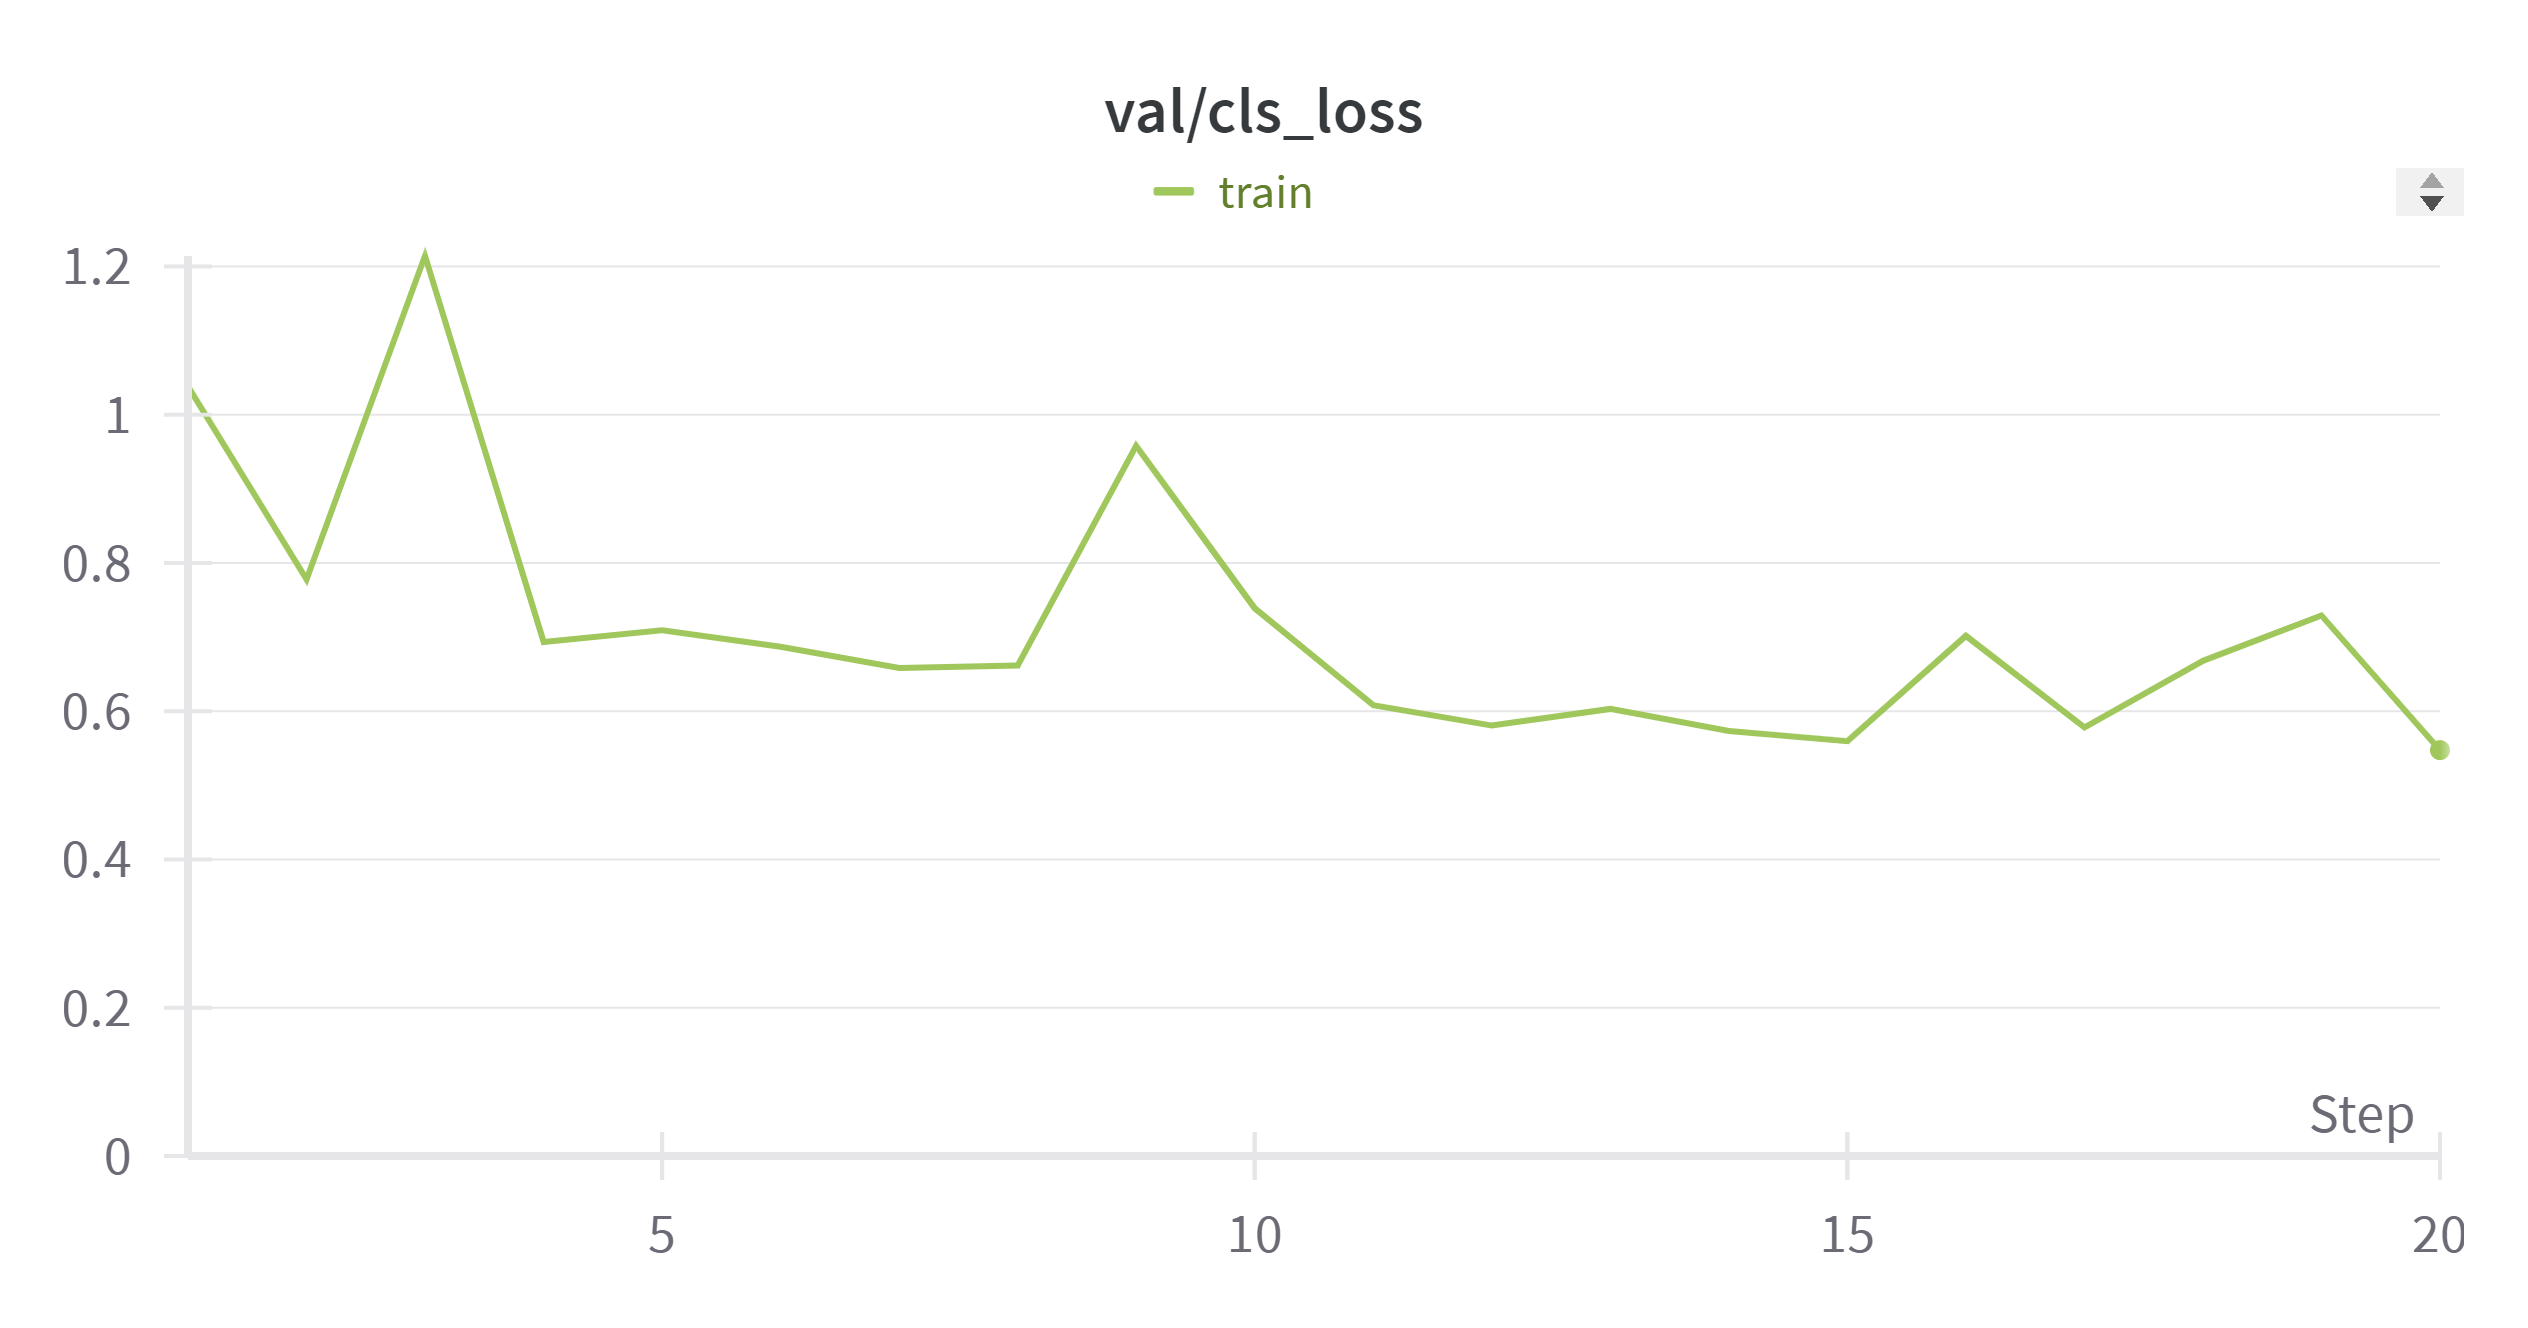
\includegraphics[scale=0.15]{img/train/val_cls_loss.png}
    \caption{Графики потерь}
    \label{cls_loss_graph}
\end{figure}

\begin{figure}
    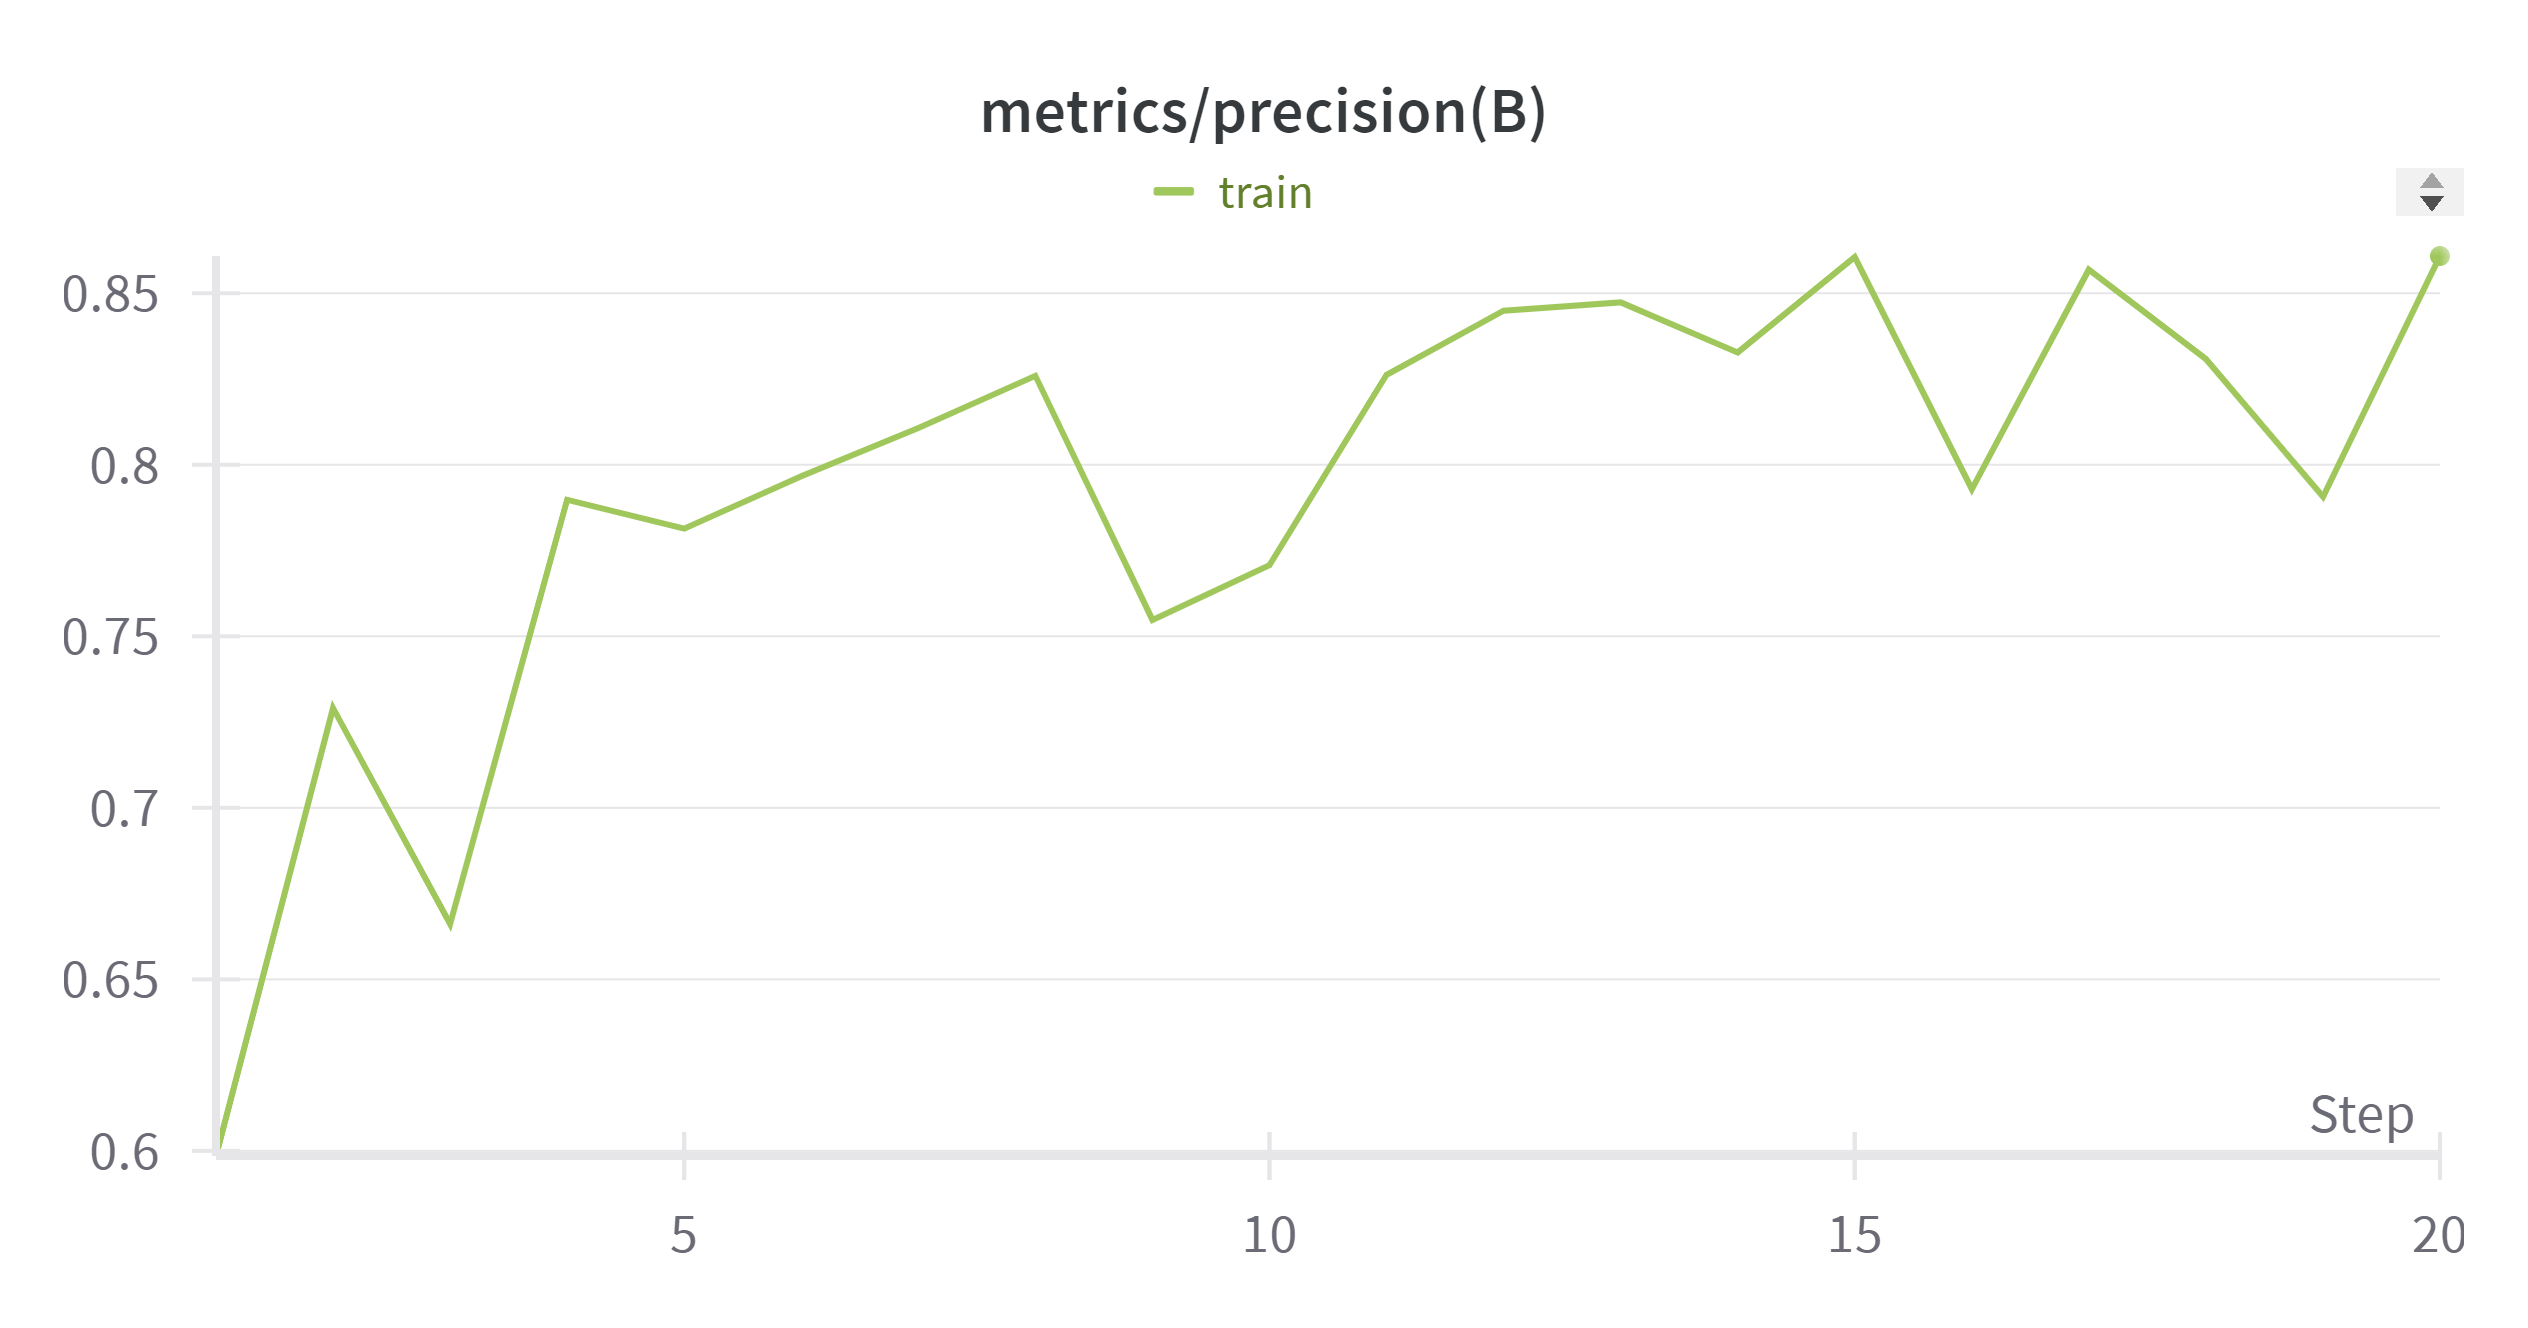
\includegraphics[scale=0.15]{img/train/precision.png}
    \caption{График точности}
    \label{precision_graph}
\end{figure}

\begin{figure}
    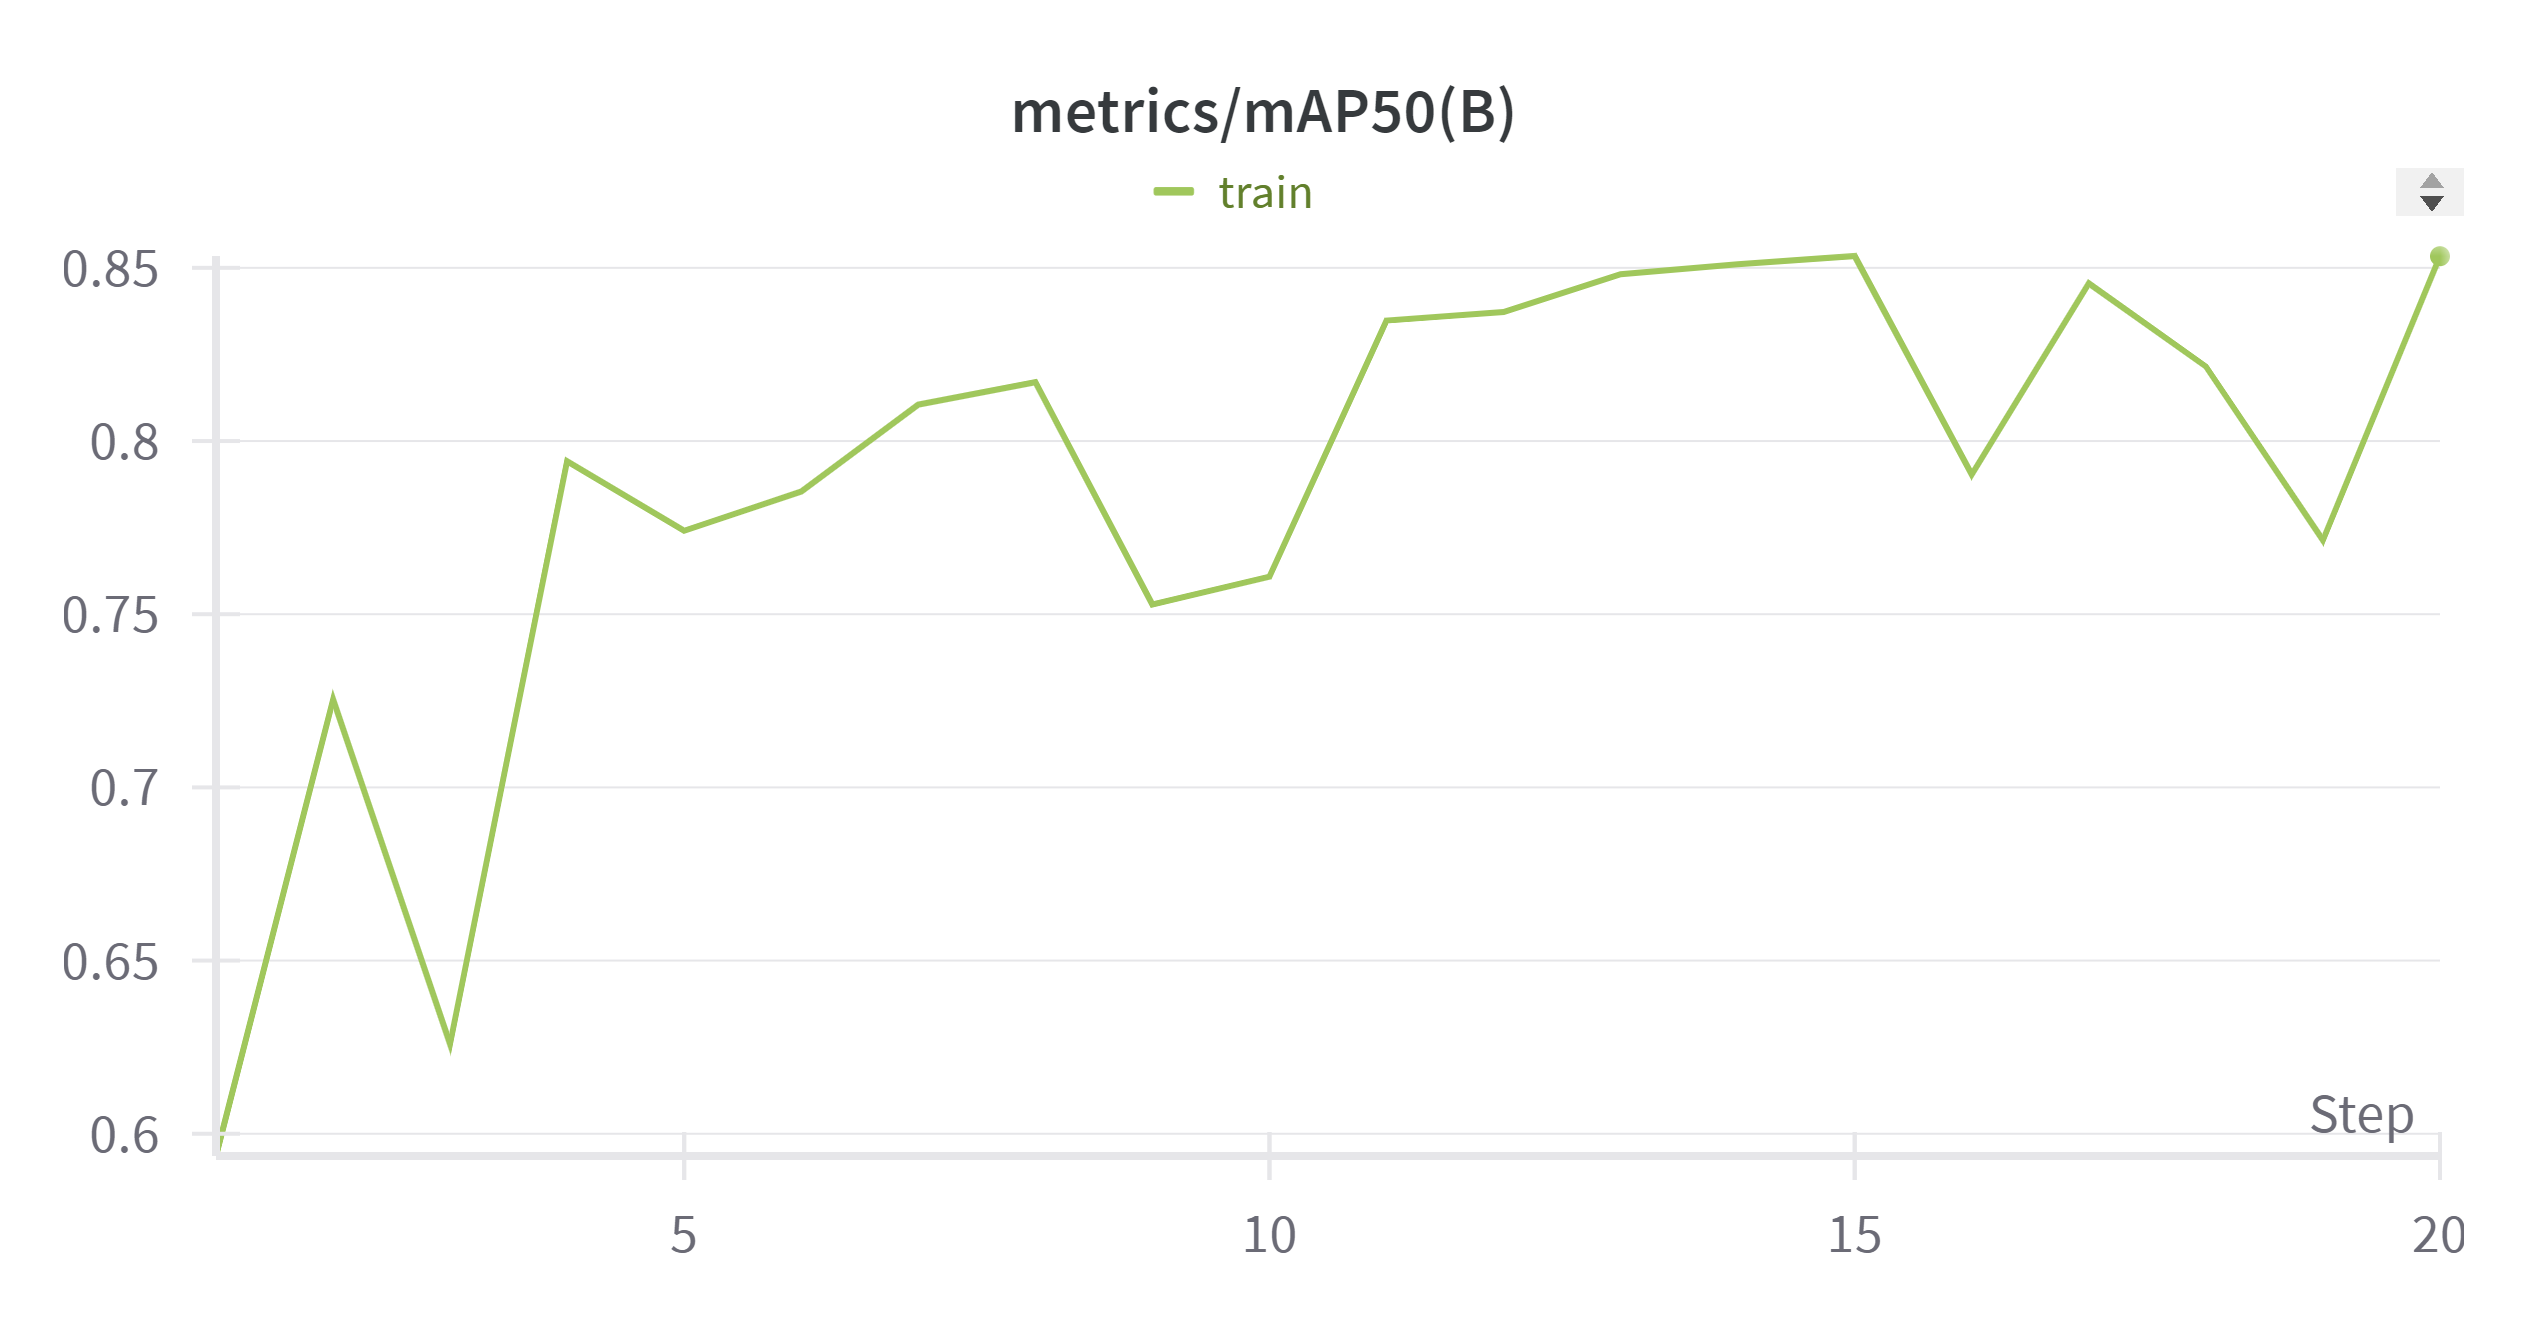
\includegraphics[scale=0.15]{img/train/map_50.png}
    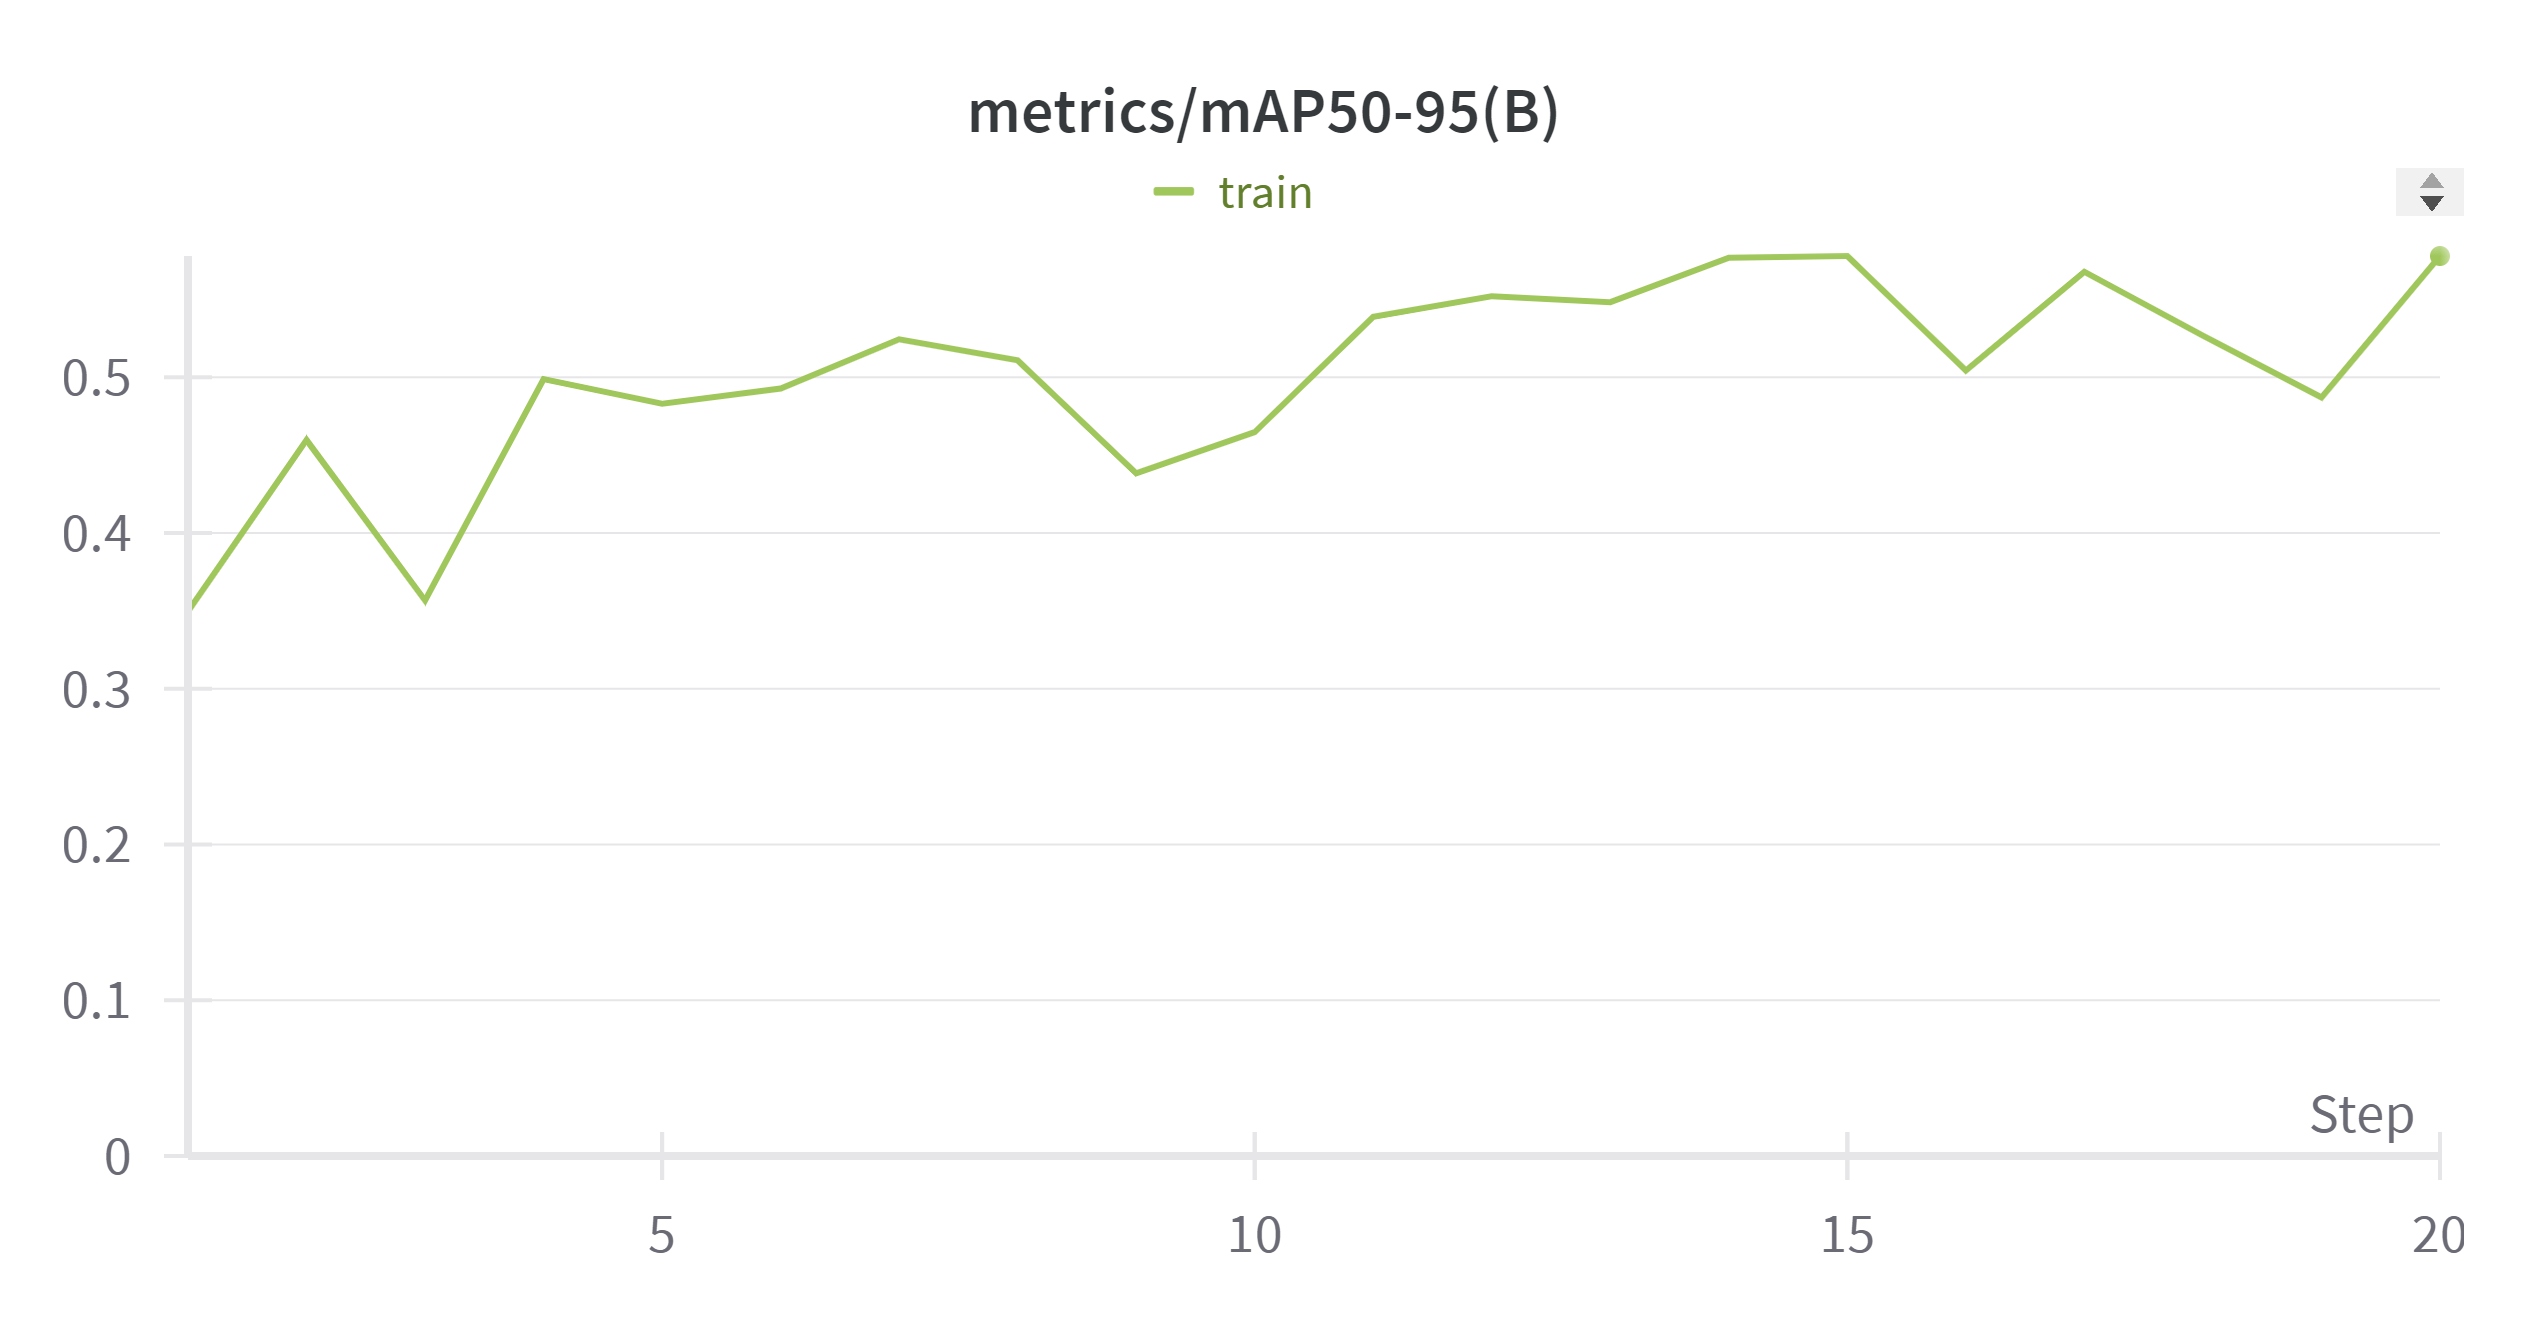
\includegraphics[scale=0.15]{img/train/map50_95.png}
    \caption{Графики $mAP$}
    \label{map_graph}
\end{figure}

На каждом из графиков ~\ref{cls_loss_graph}--~\ref{map_graph} по оси $oX$ отложен номер шага, на котором снимались показатели. Весь этап обучения, состоящий из $N$ эпох равномерно делится на $20$ этапов. На каждом этапе снимаются метрики, попадающие в результирующий график.

После обучения модель была протестирована на тестовых изображениях. На рисунках ~\ref{train_test_1} и ~\ref{train_test_2} показаны результаты тестирования.

\begin{figure}
    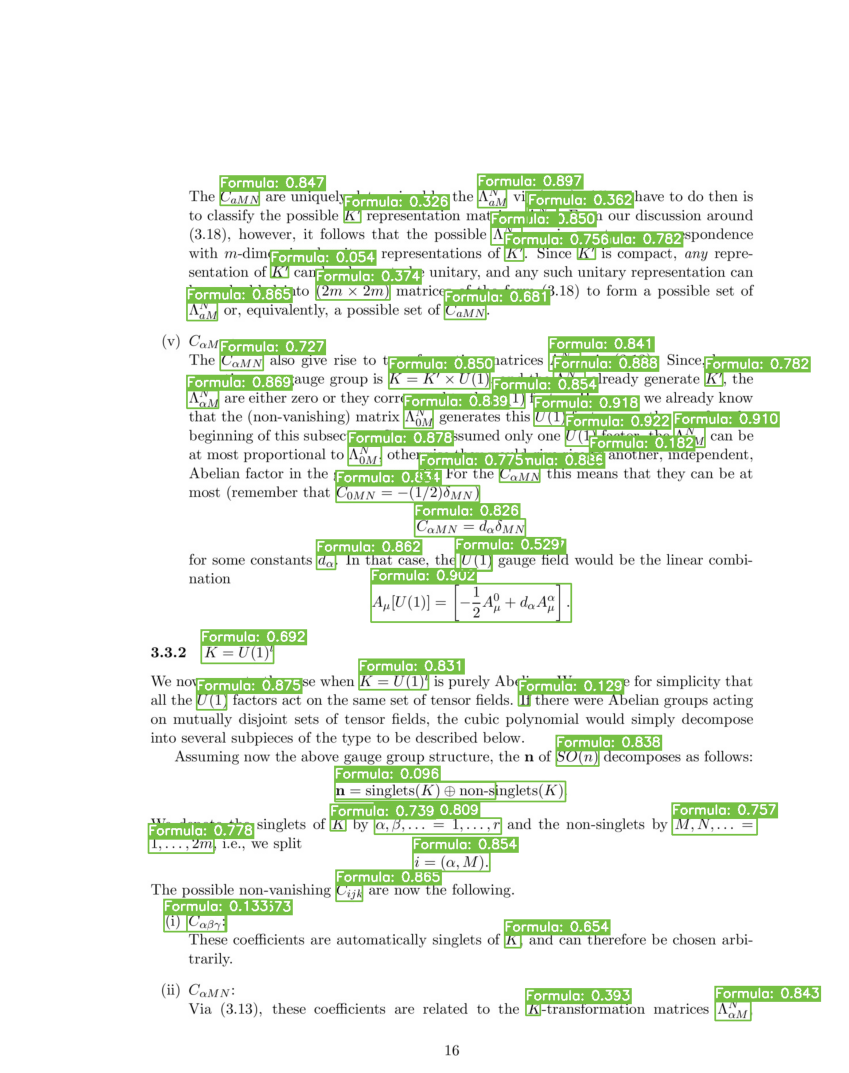
\includegraphics[scale=0.75]{img/train/test_1.png}
    \caption{Предсказание модели на тестовом изображении}
    \label{train_test_1}
\end{figure}

\begin{figure}
    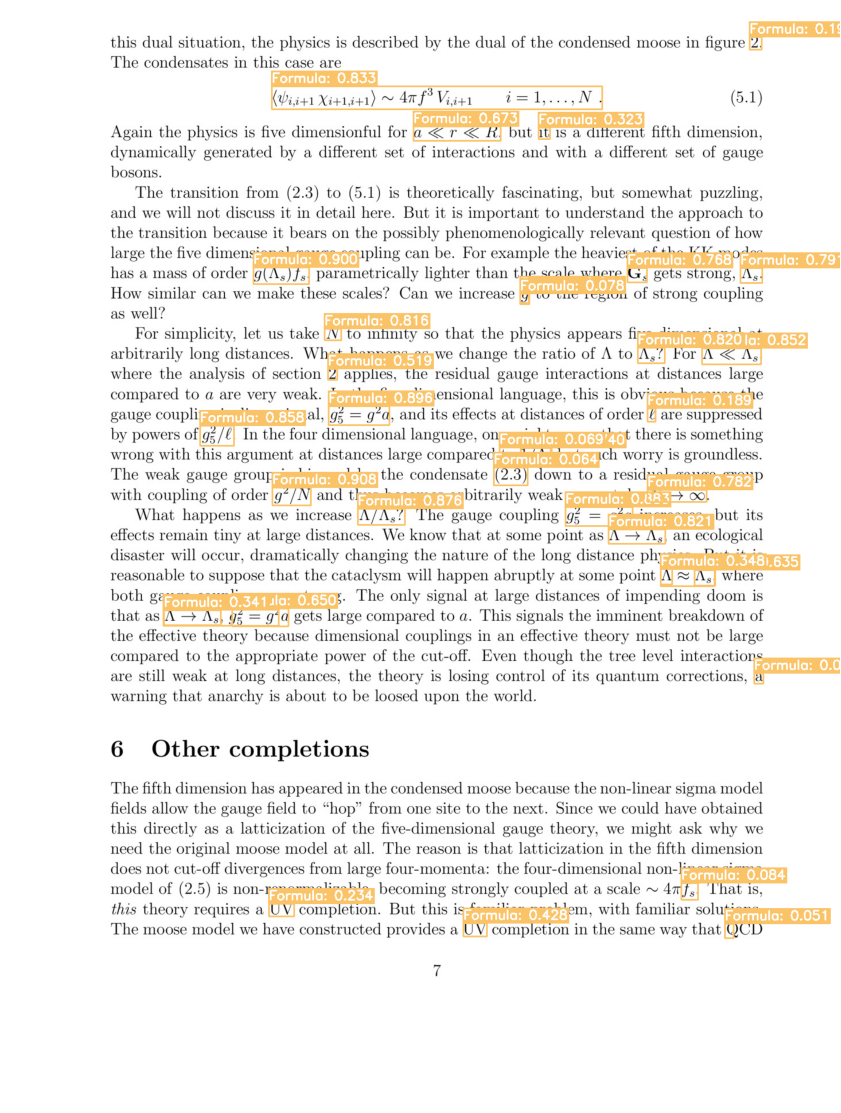
\includegraphics[scale=0.75]{img/train/test_2.png}
    \caption{Предсказание модели на тестовом изображении}
    \label{train_test_2}
\end{figure}

\subsubsection{Корректировка результата}
Как видно на рисунке ~\ref{train_test_1}, некоторые найденные формулы пересекаются друг с другом или находятся одна внутри другой. Для устранения этого дефекта используется алгоритм $\textit{NMS (Non-Maximum Suppression)}$ \cite{nms}, который реализован в $PyTorch$.
Так, например, на рисунке ~\ref{nms_img} показан результат применения алгоритма к изображению, представленному на рисунке ~\ref{train_test_1}.

\begin{figure}
    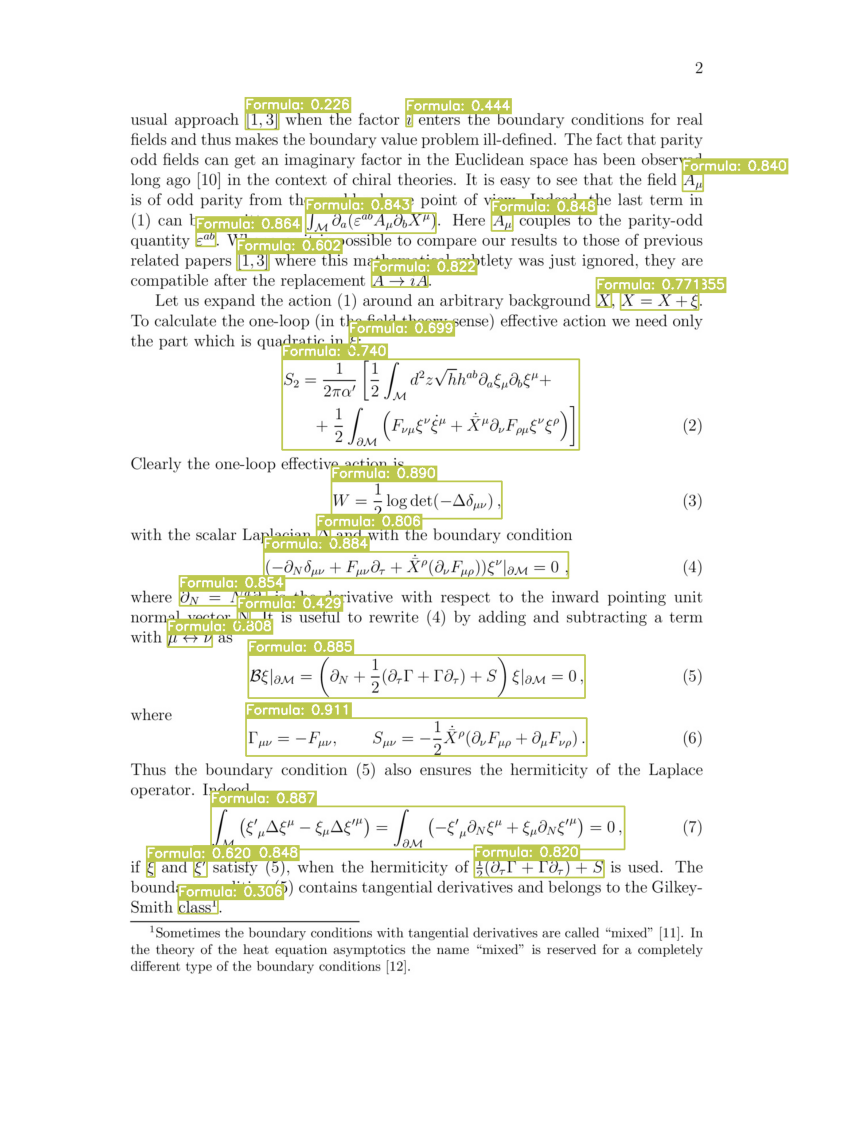
\includegraphics[scale=0.65]{img/train/nms.png}
    \caption{Скорректированное с помощью алгоритма $NMS$ предсказание модели}
    \label{nms_img}
\end{figure}